\documentclass[chap]{thesis}

% geometry
% use option 'showframe' for neatness
\usepackage{geometry}
\geometry{
left=1in,
right=1in,
top=1in,
bottom=1in}

% citations
\usepackage{cite}
\usepackage{notoccite}
\bibliographystyle{IEEErpi}
\renewcommand{\bibname}{}
\usepackage{tabularx}
% captions
\usepackage[
  labelsep=period,
  justification=centering]{caption}
\usepackage{subcaption}

% put captions above tables
\usepackage{float}
\floatstyle{plaintop}
\restylefloat{table}

% COMMAT
\usepackage{textcomp}
\usepackage{float}
\usepackage{caption}
\usepackage{multirow}
\usepackage{booktabs}
\usepackage{tikz}
\usetikzlibrary{shapes,arrows}

\tikzstyle{line} = [thick,->,>=stealth]

%\tikzstyle{line} = [draw, -latex']
\tikzstyle{decision} = [diamond, draw, fill=green!30, 
    text width=10em, text badly centered, inner sep=0pt]
\tikzstyle{process} = [rectangle, draw, fill=orange!30, 
    text width=10em, text centered, rounded corners, minimum height=5em]
\tikzstyle{input} = [rectangle, draw, fill=blue!30, 
    text width=10em, text centered, rounded corners, minimum height=5em]
\tikzstyle{block} = [rectangle, draw, fill=none, 
    text width=10em, text centered, rounded corners, minimum height=5em]
\tikzstyle{line} = [draw, -latex']

\usepackage{adjustbox}
\usepackage[justification=centering]{caption}


% mathematics
\usepackage{amsmath}
\usepackage{amssymb}
\usepackage{amsthm}
\usepackage{mathrsfs}
\usepackage{upgreek}

% figures
\usepackage{graphicx}

% make things pretty
\usepackage{color}
\usepackage[hidelinks]{hyperref}

% make pretty graphs
\usepackage{tikz}
\usetikzlibrary{arrows}

% make pretty tables
\usepackage{tabu}
% algorithms
\usepackage{algpseudocode}
\usepackage{algorithm}
\usepackage{longtable}
% code listings
\usepackage{listings}
\lstdefinestyle{mystyle}{
  basicstyle=\ttfamily,
  language=C++,
  columns=fullflexible,
  keepspaces=true,
  numbers=left,
  xleftmargin=2em
}

% conform to IEEE
\renewcommand{\captionfont}{\bfseries}
\renewcommand{\figurename}{Fig.}
\renewcommand*{\UrlNoBreaks}{\do\(\do\[\do\{\do\<\do\:}%

% href for toc
\makeatletter
\usepackage{etoolbox}
\pretocmd{\tableofcontents}{%
  \if@openright\cleardoublepage\else\clearpage\fi
  \pdfbookmark[0]{\contentsname}{toc}%
}{}{}%
\makeatother

% theorems and propositions
\newtheorem{prop}{Proposition}
\theoremstyle{remark}
\newtheorem{rmk}{Remark}

% make typing easier
\newcommand{\B}{\mathcal{B}}
\newcommand{\E}{\mathcal{E}}
\newcommand{\G}{\mathcal{G}}
\newcommand{\I}{\mathcal{I}}
\newcommand{\J}{\mathcal{J}}
\newcommand{\R}{\mathcal{R}}
\newcommand{\V}{\mathcal{V}}
\newcommand{\OP}{\mathcal{L}}
\renewcommand{\H}{\mathcal{H}}
\renewcommand{\O}{\mathcal{O}}
\renewcommand{\P}{\mathcal{P}}
\renewcommand{\S}{\mathcal{S}}
\newcommand{\bs}[1]{\boldsymbol{#1}}

% make editors mad - keep my sanity
\renewcommand{\bar}[1]{\overline{#1}}
\renewcommand{\tilde}[1]{\widetilde{#1}}
\newcommand{\paira}[2]{\,{}_{\V^*}^{}\!\left< {#1}, {#2} \right>_{\V}}
\newcommand{\pairb}[2]{\,{}_{\V}^{}\!\left< {#1}, {#2} \right>_{\V^*}}
\newcommand{\adv}[1]{-\kappa \nabla^2 {#1} + \bs{a} \cdot \nabla {#1}}
\newcommand{\madv}[1]{\kappa \nabla^2 {#1} - \bs{a} \cdot \nabla {#1}}
\newcommand{\adva}[1]{-\kappa \nabla^2 {#1} - \bs{a} \cdot \nabla {#1}}
\newcommand{\madva}[1]{\kappa \nabla^2 {#1} + \bs{a} \cdot \nabla {#1}}

\begin{document}
\thesistitle{\bf Machine learning based Reduction and Quantification of Error in Image Classification Pipelines}

\author{Aritra Chowdhury}
\degree{Doctor of Philosophy}
\department{Computer Science}
\submitdate{[August 2018] \\ Submitted June 2018}
\copyrightyear{2018}

\titlepage
\copyrightpage
\tableofcontents
\listoftables
\listoffigures

\specialhead{ACKNOWLEDGMENT}

I would first of all like to thank my parents, Arindam Chowdhury and Babli Chowdhury for everything. I am here because of them and anything I do will never be enough to repay the sacrifices that they made for me. It is an honour to be their son. They have supported me in my journey through thick and thin and I am very grateful for everything that they have done for me.

I would like to specially  thank my adviser, Prof. B{\"u}lent Yener for guiding me throughout my Ph.D. His advice about everything, starting from the projects that we have worked on together, to how to navigate life in the academic world, has proved to be invaluable. It has been
a wonderful learning experience for me to have had the opportunity to work with
him these past 5 years. He has been a role model for me and many others with his professionalism, openness, caring attitude, and big heart. 
I would  like to thank my committee members - Prof. Malik Magdon-Ismail, Prof. Charles Stewart and Dr. Alberto Santamaria-Pang for helping me with the thesis and guiding me in the right direction.  I am grateful that I have had the opportunity to work with  Prof.  Magdon-Ismail, Prof. Dan Lewis and Dr. Santamaria-Pang, and learn immensely from them.


I would also like to show my gratitude to my friends and colleagues here at RPI. It was a lot of fun discussing about research and life with my friends and colleagues (Kshiteesh Hegde, Maksim Tsikhanovich, Nivas Nambirajan, Nimit Dhulekar, Haidar Khan, Elizabeth Kautz, Daniel Park, Gilna Samuel, John Postl, Anik Saha).
I would also like to specially thank my roommates Atriya Sen and Partha Sarathi Mukherjee who have proved to be my family away from home.


I would also like to acknowledge the staff at Lally - Christine Coonrad, the late Terry Hayden (who we all miss very much), Mike (the environmental specialist), Tracy Hoffman and others. I would like to thank you for making our work life easy. 

This section would be incomplete without mentioning certain establishments like First Choice Carribean, Red and Blue and Snowman's ice cream. They have been a source of joy and nourishment throughout the years of my Ph.D.
\specialhead{ABSTRACT}

Image classification is an approach of pattern recognition in computer vision. The objective is to differentiate between different classes of images based on the quantification of contextual information in the imagesand it is performed using data analytic pipelines. These pipelines are organized as interdependent and individual components. The components include image acquisition, image preprocessing, feature extraction, feature preprocessing, dimensionality reduction and learning algorithms among others. More steps may be added or removed from the pipeline. The quality of the image classification pipeline is measured by the validation error or test error in classification of unseen image instances that quantify the generalization error. Even though the error appears as a result of application of the learning algorithm, it is actually an accumulation of the errors introduced from different parts of the pipeline starting from the acquisition of the image from the sample, the feature preprocessing algorithms, the feature extraction algorithms and finally to the learning algorithm used for performing the  classification. This error is propagated down the pipeline which is finally accumulated in the form of the aforementioned classification error. In this dissertation, we attempt to holistically optimize, quantify and understand the contribution of error from the various components of image classification pipelines.   


The first work involves an image classification problem in the domain of blood vessel characterization. Here we show how optimizing a particular component of the pipeline, in particular data pre-processing, reduces the classification error. The objective is to differentiate between vascular morphologies occurring in fluorescence microscopic 2D samples of neuropathological tissue samples. The main source of error in this problem arises as a result of imbalance in the training dataset. We address this problem by modeling artificial parametric 3D models of blood vessels to augment the training dataset and reduce the imbalance in the dataset. Pre-trained convolutional neural networks are used as the feature extraction algorithm in this work. We show that a combination of the artificial and natural data increases the accuracy of classification and as a result reduces the generalization error.

In the second work, we minimize the error in image classification pipelines. Here we show how we can reduce the classification error by considering the pipeline as a whole instead of optimizing individual components. The problem selected for demonstrating this is that of automatic microstructure recognition. The dataset for this problem is from the domain of material science. It consists of images of microstructures in the micrometer scale. We perform two classification tasks. The first task is of differentiating between dendritic and non-dendritic microstructures. The second task is of differentiating between longitudinal and transverse cross sections of microstructures. The objective for both the classification tasks is to find the best set of algorithms and hyper-parameters for minimizing the classification error. The approach used was an exhaustive grid search of the configuration space of algorithms and corresponding hyper-parameters for three stages of the pipeline - feature extraction, dimensionality reduction and learning algorithms. This exhaustive grid search is able to perform classification of the two tasks with a sufficiently high degree of accuracy. We demonstrate that pre-trained convolutional neural networks along with support vector machines with a linear kernel can be used for characterizing microstructures. In addition, we also show that exhaustive grid search based methodology can be used for finding the best algorithms and hyper-parameters for the problem of microstructure recognition in the domain of material science.

In the second part of the Thesis, we try to understand the  error contributions from different components of  image classification pipelines. In the first work of this part, we are trying to quantify the quality of the individual image samples and also of the  entire dataset. This involves the computation of a score to quantify the quality of an image sample. This score is computed by leveraging the probabilities of machine learning algorithms. The dataset is annotated by a pathologist as \textit{good} or \textit{bad} depending on whether it has high or low amount of signal. Texture based features are used to extract information from the images. Classification algorithms are used to classify the data. This score therefore provides a way to filter a dataset based on the quality of the image samples.

The final work involves a proposal of methods to quantify the contribution of errors in image classification pipelines. In particular, we propose an \textit{agnostic} methodology to compute the contribution of errors from different components of the image classification pipeline.  We show that algorithm selection and hyper-parameter optimization algorithms maybe used for error quantification. We empirically demonstrate that random search can efficiently and accurately quantify the contribution of errors from different components  in image classification pipelines.



%%% INTRODUCTION AND BACKGROUND
\chapter{INTRODUCTION AND BACKGROUND}
\label{chap:intro}

%%% OUTLINE
\section{Outline}


%%% CONTRIBUTIONS
\section{Contributions}


%\include{automated}
\chapter{IMAGE DRIVEN MACHINE LEARNING METHODS FOR MICROSTRUCTURE RECOGNITION}
\label{chap:COMMAT}

\let\thefootnote\relax\footnotetext{
This chapter previously appeared as:
A. Chowdhury, E. Kautz, B. Yener, and D. Lewis. "Image driven machine learning methods for microstructure recognition."  \emph{Computational Materials Science}, vol. 123 pp. 176-187, 2016.}



%%% INTRODUCTION
\section{Introduction}
\label{intro}

This is the first chapter in the error optimization part of the thesis. In this chapter, we attempt to minimize the error of classification in the problem of microstructure characterization. In this chapter, we are optimizing the components of an image classification pipeline as a whole as shown in Fig. \ref{fig:chapter3}.

\begin{figure}[ht!]
\centering
\includegraphics[width=1.0\textwidth]{img/chapter3}
\caption{Reducing classification error by optimizing the components of the image classification pipeline together instead of in isolation. The steps in the image classification pipeline highlighted in red are optimized simultaneously to minimize the classification error.}
\label{fig:chapter3}
\end{figure}

 Materials characterization is a critical aspect of the material design and discovery process.  Recently, there has been much research in the field of materials informatics, a growing research area in which information technology and data science methods are used to interpret and analyze material data in order to accelerate the material discovery, design, and development process \cite{XuH2015, Rodgers2006, Broderick2008, ferris2007materials, Kalidindi2011}.  Currently, material design relies on chance discoveries and follows a classical synthesis-characterization-theory-computation approach \cite{SergeiV.Kalinin2015}.  Further, there is a heavy reliance on individual researcher background and experience which introduces significant bias and potentially error into the process of microstructure recognition, interpretation, and characterization. 
%
For example, quantification of microstructures traditionally is done using stereological measurements.  Bias is introduced into stereological measurements through the requirement that an expert must first recognize and identify key microstructural features (inclusions, grains, or phases).  This bias can be caused by a variety of factors, such as an individual's background, education, and experiences \cite{SergeiV.Kalinin2015}.  

Although there have been recent advances in the field of quantitative microstructural science, there is still a heavy dependence on expert knowledge to identify what microstructural features are of interest for quantification \cite{DeCost2015}. Therefore it is desirable to expand upon work previously presented by DeCost and Holm in Reference \cite{DeCost2015}, and further explore methods of quantitative microstructure representations which do not require \textit{a priori} knowledge of microstructural features of interest or significance \cite{SergeiV.Kalinin2015}. This work aims to leverage existing computer vision and machine learning techniques specifically for the challenge of microstructure recognition.  While the overlap between computer vision, machine learning, and materials science is currently small \cite{SergeiV.Kalinin2015}, this work is a step towards increasing cross-disciplinary studies that challenge the current paradigm for microstructure characterization. 
%

Dendritic morphologies were chosen for this small case-study since dendrites are a well-characterized microstructural feature that exists in a variety of material systems (from single to multi-component).  Size, shape, and spacing of dendrites vary depending on solidification behavior and chemistry, thus micrographs of this single feature can vary widely.  The sample preparation and imaging methods used also contribute to the variety of micrographs produced from dendritic microstructures. Despite this variability in image data, it is still possible for human experts to look at a micrograph that contains dendrites and identify that it contains this microstructural feature, even though different orientations of dendrites (transverse or longitudinal) look distinctly different.  

Computer vision and machine learning methods were applied to the task of identifying a particular microstructural feature of interest (dendrites) from micrographs that do not contain this particular feature (just as a human expert would identify that a micrograph contains dendrites).  This recognition task is referred to in this work as Task 1.  Task 1 is a high-level microstructure recognition task in the sense that dendrites are a type of microstructural feature that are not specific to a material system.  A second classification task (referred to here as Task 2) was also completed, and involved distinguishing between longitudinal and transverse cross-sectional views of dendritic microstructures. This task may be viewed as a logical next step following the identification of dendrites in Task 1.

The contribution in this work is to investigate multiple computer vision and machine learning methods for microstructure recognition. We hypothesize that the approach and methods presented here can be generalized, and thus applied to a variety of microstructure recognition tasks that act as a necessary first step in characterization of a material system.
%-----------------------------------------

\section{Alloy Fabrication and Sample Preparation}
\label{sample_prep}

The alloy fabrication, processing, and metallographic sample preparation procedure followed to obtain images used in this work was based on the process detailed in References \cite{Schaefer2005} and \cite{Mao2014} and is summarized here. 
%

A Materials Research Furnaces (MRF) three probe arc melter was used to fabricate alloys of varying Sn-Ag-Cu compositions.  After melting alloys were allowed to solidify and were then prepared for directional solidification (DS).  The solidified buttons were placed in a beaker on a hot plate.  The button was re-melted while constantly being purged with Ar gas to minimize sample oxidation. The alloy melt was then transferred into a 4 mm inner diameter quartz ampule with a mechanical pump.  The rods were allowed to cool, then removed from the ampule, and placed in a larger quartz ampule (5 mm inner diameter) for DS.  This ampule was then back-filled with Ar gas, sealed using a hydrogen torch, and inserted into the DS furnace.

DS was performed using a Bridgman-type apparatus in order to refine alloy microstructure.  The tube furnace in this apparatus is a Thermolyne Type-21100 fitted with an Omega temperature controller.
Following DS, alloys were removed from the quartz ampule, and small sections from the middle third of the rod were mounted in epoxy for metallographic sample preparation.  Sections were mounted such that transverse and longitudinal orientations of $\beta$-Sn dendrites could be viewed.  Samples were ground using silicon carbide (SiC) papers to 600 grit, then polished using 9, 3, and 1 $\mu$m diamond slurries.  Colloidal silica was used as the final polishing step and as a chemical etchant so that the dendritic microstructure would be readily visible using light optical microscopy.

%----------------------------------------------------------------------------------
\section{Image Data Sets}
\label{data_sets}

Image data used in this study includes micrographs taken over a span of approximately three years by students in the Lewis Research Group in the Materials Science and Engineering Department at Rensselaer Polytechnic Institute (RPI).  All images taken by Lewis Research Group members are of solder alloys with dendritic microstructures.  These alloys were manufactured, processed, and imaged at RPI, and a representative process of sample preparation was presented in Section \ref{sample_prep}.  In order to supplement micrographs obtained at RPI, micrographs from the publicly available Dissemination of Information Technology for the Promotion of Materials Science (DoITPoMS) library \cite{Barber2003} were used. Example images used in classification are provided in Figure \ref{fig:example_images}.   

Images were grouped into two data sets: Data Set 1 and Data Set 2, corresponding to classification Tasks 1 and 2 respectively. Data Set 1 is comprised of micrographs with and without dendritic morphologies.  This data set includes all images with dendrites (longitudinal and transverse cross-sections) from both the Lewis Group and the DoITPoMS micrograph library \cite{Barber2003}.  All micrographs that do not depict dendritic morphologies were obtained from the DoITPoMS library.  Data Set 1 includes 528 images that are each 227 by 227 square pixels. 264 original images were used in making Data Set 1 (132 micrographs containing dendrites and 132 micrographs without dendrites). Each original image is 270 by 500 pixels but includes a scale bar that interferes with feature extraction, therefore each image was cropped to yield two 227 by 227 square pixel images.  Thus, 528 images were used for classification. 

Data Set 2 is a subset of Data Set 1, and is comprised of micrographs that only contain dendrites, where each micrograph is either a transverse or longitudinal cross-sectional view.  Micrographs used in this data set include both images from the Lewis Group and the DoITPoMS micrograph library.  Data Set 2 contains a total of 188 images that are each 227 by 227 square pixels. As was done for Data Set 1, original images were cropped to remove the scale bar: 47 micrographs of each longitudinal and transverse sections (total of 94 original images) were cropped to create a 188 images used for classification.
%
\begin{figure}
  \begin{centering}
 \includegraphics[scale=0.55]{img/example_images_v2.png}
 \caption{Examples of micrographs used in classification.  Micrographs shown in (a) and (b) are longitudinal and transverse cross-sectional views of dendrites, whereas micrographs in (c) do not contain dendrites.  Micrographs in (a), (b) and (c) were used in Task 1, and micrographs in (a) and (b) were used in Task 2.}
 \label{fig:example_images}
 \end{centering}
\end{figure}
%-----------------------------------------
\section{Approach}
\label{approach}
%
The general approach applied to the task of micrograph classification involved feature extraction and feature selection (dimensionality reduction) to compute feature vectors that were then used for training, validating, and testing various classification models.  The same approach was applied to both Data Sets 1 and 2 and is shown schematically in Figure \ref{fig:approach_overview}.

Feature extraction is the first step in the process of classifying micrographs.  Feature extraction starts with feature detection, where features in an image are local regions of pixels that include an `interesting' part of a microstructure, such as a corner, edge, or blob-like object. Features detected using computer vision algorithms are not necessarily semantically meaningful, however are pixel patterns that are mathematically repeatable and recognizable, thereby making the region a good feature. Detected features are then described (or represented) in the form of a vector, called a feature vector. A feature vector is comprised of a set of detected features in the image, and each image can thus be described or represented by a feature vector.  Multiple feature extraction methods were tested in this work in order to compare classification accuracies of different image representations.   
%

These feature vectors, derived in the process of feature extraction, have high dimensionality and in this work feature selection was performed after feature extraction for computational efficiency and to preclude the curse of dimensionality \footnote{The phrase `curse of dimensionality' refers to issues associated with increasing data dimensionality in Euclidean space.  Behavior of algorithms in low dimensional space, such as in three dimensions, may not generalize well to a higher dimensional space \cite{Keogh2010}.}.  Feature selection involves reducing the length of the feature vector while still retaining image information.  For example, if a feature vector is sparse, dimensionality reduction would involve reducing the sparsity of this vector.  Different dimensionality reduction methods were applied to test how each technique impacted classification accuracies.   

After feature extraction and selection, various classification models were trained, validated, and tested.  A 5 fold cross validation split was used for each data set.  This split was selected in order to minimize variance in model parameters%(determined via five-fold cross-validation on each of the 5 training folds), 
, and to avoid over-fitting.  These validation accuracies were then averaged and the standard deviation was calculated in order to evaluate model stability.  
%
\begin{figure}
  \begin{centering}
 \includegraphics[scale=0.4]{img/flowchart_approach_updated.png}
 \caption{Overview of approach used in classification of micrograph data.  The approach summarized here shows 140 different combinations of feature extraction, feature selection and classification methods completed.  The same approach presented here was completed first for Task 1 (Data Set 1), then for Task 2 (Data Set 2).}
 \label{fig:approach_overview}
 \end{centering}
\end{figure}
%
We performed analysis on the two datasets (described in Section \ref{data_sets}) in the form of two classification tasks: Task 1 and Task 2. 

%The relationship between these tasks is depicted in Figure \ref{fig:tasks_flowchart}. 

%%Flowchart made using tikz
%\begin{figure}[t!]
%\centering
%\begin{adjustbox}{width=\textwidth,height=0.75\textheight,keepaspectratio}
%\subfigure[Task 1]{
%% \centering
%\begin{tikzpicture}
%[node distance =  5cm]
%    % Place nodes
%    \node [input] (input) {Input: Micrograph};
%    \node [decision, below of=input,yshift=-2cm] (task1) {Task 1: Does the micrograph depict a dendritic microstructure?};
%    % \node [decision, below of=task1,yshift=-2cm] (task2) {Task 2: Transverse cross-section?};
%    % \node [process, below of=task2,yshift=0cm] (trans) {Transverse cross-section of dendritic microstructure};
%    \node [process, below of=task1,yshift=0cm] (dendrite) {Dendritic microstructure};
%    \node [process, right of=task1, xshift=2cm] (nondendrite) {Non-dendritic microstructure};
%    % \node [process, right of=task2, xshift=4cm] (long) {Longitudinal cross-section of dendritic microstructure};
% 
%    % Draw edges
%   \path [line] (input) -- (task1);
%%   \path [line] (task1) -- node [anchor=east] {yes} (task2);
%  \path [line] (task1) -- node [anchor=east] {yes} (dendrite);
%   \path [line] (task1) -- node [anchor=south]{no} (nondendrite);
%%   \path [line] (task2) -- node [anchor=south]{no} (long);
%
%\end{tikzpicture}
%}
%
%\subfigure[Task 2]{
%% \centering
%\begin{tikzpicture}
%[node distance =  5cm]
%    % Place nodes
%    \node [input] (input) {Input: Dendritic Micrograph};
%    % \node [decision, below of=input,yshift=-1cm] (task1) {Task 1: Does the micrograph depict a dendritic microstructure?};
%    \node [decision, below of=input, yshift=-2cm] (task2) {Task 2: Transverse cross-section?};
%    \node [process, below of=task2,yshift=0cm] (trans) {Transverse cross-section of dendritic microstructure};
%    
%    % \node [process, right of=task1, xshift=4cm] (nondendrite) {Non-dendritic microstructure};
%    \node [process, right of=task2, xshift=2cm] (long) {Longitudinal cross-section of dendritic microstructure};
% 
%    % Draw edges
%   \path [line] (input) -- (task2);
%%   \path [line] (task1) -- node [anchor=east] {yes} (task2);
%   \path [line] (task2) -- node [anchor=east] {yes} (trans);
%%   \path [line] (task1) -- node [anchor=south]{no} (nondendrite);
%   \path [line] (task2) -- node [anchor=south]{no} (long);
%
%\end{tikzpicture}
%}
%\end{adjustbox}
%\caption{Flowchart of microstructure recognition tasks, referred to here as Task 1 and Task 2.  Tasks 1 and 2 are both binary classification tasks. (a) Task 1 involves distinguishing between micrographs that depict dendritic morphologies from those that do not contain this particular microstructural feature.  (b) Task 2 involves distinguishing between different cross-sectional views (longitudinal or transverse) of dendritic microstructures.}
%\label{fig:tasks_flowchart}
%\end{figure}
%----------------------------------------------------------------------------------
\section{Computer Vision and Machine Learning Methods}
\label{methods}

As previously introduced in Section \ref{approach}, multiple feature extraction and selection methods were tested with various classifiers in order to evaluate the best methods to apply to microstructure recognition tasks.  The methods applied in this work are discussed in additional detail in Sections \ref{feature_extraction} - \ref{classification}.  Additionally, Section \ref{related_work} provides a brief overview of computer vision and machine learning methods applied to other research in the field of materials science. 

\subsection{Feature extraction}
\label{feature_extraction}

Feature extraction methods applied in this work are texture and shape statistics (which include Haralick texture features \cite{Haralick1973}, histogram of oriented gradients (HoG) \cite{Dalal2005}, local binary patterns (LBP) \cite{Ojala2002}, Hu moments \cite{Hu1962,Otsu1975}, Zernike Moments \cite{Khotanzad1990},threshold adjacency statistics \cite{Lievers2004}), visual bag of words (VBOW) \cite{Yang2007,Bay2006}, and pre-trained convolutional neural networks (CNN's).  We used the publicly available Caffe framework \cite{Jia2014} for all experiments involving pre-trained CNN's. The network was based on the architecture of Krizhevsky \textit{et al.} for ImageNet \cite{Krizhevsky2012}.  The approach of using a pre-trained network was taken in this case-study because this is a good first step that does not require training to determine model parameters, which would be a difficult task with the small data sets used in this study \cite{Jia2014}. 
  
Texture and shape statistics involve multiple feature extraction algorithms (previously listed) that operate on image texture and shape of objects within the image.  These methods are introduced below:   

Haralick features \cite{Haralick1973} are calculated using gray-level co-occurrence matrices (\textit{G$_{ij}$}, shown below) which are square matrices of size \textit{N$_g$} x \textit{N$_g$}, where \textit{N$_g$} is the number of gray levels in an image:
\\
\begin{equation}
%\[
G_{ij}=
  \begin{bmatrix}
    p(1,1) & p(1,2) & \cdots       & p(1,N_{g}) \\
    p(2,1) & p(2,2) &  \cdots      & p(2,N_{g}) \\
     \vdots &  \vdots &  \ddots    &  \vdots          \\
    p(N_{g},1)  & p(N_{g},2) & \cdots & p(N_{g},N_{g}) 
  \end{bmatrix}
%\]
\end{equation}
\\
Each matrix element, $ \ [i,j]\ $, is calculated by counting the number of times a pixel with value \textit{i} is adjacent to pixel with value \textit{j}.  When considering a square pixel image, there are four directions for which a gray-level co-occurrence matrix can be calculated: horizontal, vertical, left diagonal, and right diagonal.  Haralick texture statistics can be calculated based on the four gray-level co-occurrence matrices from each of these four directions. Haralick features thus describe the texture of an image. Fundamentally, texture is the arrangement of a certain feature or property, relative to the environment. In images, texture is the spatial distribution (arrangement) of gray-level variations in an image. Haralick features, computed from image gray-level co-occurrence matrices, capture texture patterns in an image. 

The histogram of oriented gradients (HoG) \cite{Dalal2005} method describes an image with a set of histograms of gradient orientations from local regions of an image (referred to as cells).  Each histogram reports the number of times a gradient orientation occurs in a given cell.  In general, an image gradient is a two-vector that points in the direction of the greatest rate of change.  The two components in the gradient vector include the gradient magnitude, $M(x,y)$, and the gradient orientation, $\alpha$$(x,y)$: 

\begin{equation}
%\[ M(x,y) = \sqrt{g_{x}^2+g_{y}^2} \]
M(x,y) = \sqrt{g_{x}^2+g_{y}^2}
\end{equation}
%\\
\begin{equation}
%\[ \alpha(x,y) = \tan^{-1}({\frac{g_{x}}{g_{y}}})\]
\alpha(x,y) = \tan^{-1}({\frac{g_{y}}{g_{x}}})
\end{equation}
\\
where $g_{x}$ and $g_{y}$ are the x and y components of the gradient respectively.  The normalized histograms of each cell are concatenated to form a descriptor vector for each image.  The greater the number of bins, the more detailed the histogram, and thus feature vector.

Local Binary Patterns (LBP) \cite{Ojala2002} method also describes the texture of an image.  Each image is split into cells and the neighborhood of each pixel (in each cell) is thresholded.  The neighborhood surrounding each pixel is defined by the pixel's eight nearest neighbors. When the center pixel intensity value is greater than its neighbor, the pixel value is changed to 0, otherwise the pixel value is 1. For each pixel, an 8-digit binary number, which can be referred to here as a label, is created. A histogram is created for each cell that reports the frequency of each label. The histograms for each cell are normalized, then all histograms are concatenated to yield a feature vector for the entire image. 

%A label is assigned by the operator to every pixel of an image by thresholding the neighborhood of each pixel with the center pixel value and using this result as a binary number. The local neighborhood is defined as a set of sampling points evenly spaced on a circle centered at the pixel to be labeled. Interpolation techniques are used when a sampling point does not fall on the center of the pixel.
%---------------------------------------------------------------------------------------------------------
Hu moments \cite{Hu1962,Otsu1975} are shape-based feature descriptors that describe, characterize, and quantify shapes of objects in an image.  
Hu moments are based on geometric moments, defined by $m_{p,q}(x,y)$: 

\begin{equation}
%\[ 
m_{p,q}(x,y) = \int_{-\infty}^{\infty} \int_{-\infty}^{\infty} x^{p} y^{q}f(x,y) dxdy
%\]
\end{equation}
\\
Since images are a collection of pixels, the moment of an image must be expressed in terms of summations instead of integrals, as follows: 
\begin{equation}
%\[ 
m_{p,q}(x,y) = \sum_{-\infty}^{\infty} \sum_{-\infty}^{\infty} x^{p} y^{q}f(x,y) dxdy
%\]
\end{equation}
\\

From the above equation, the area of an image would simply be defined by the 0th moment.  The centroid of an image can also be defined using this concept of geometric moments, as follows: 
\begin{equation}
%\[ 
(\bar{x},\bar{y}) = (\frac{m_{10}}{m_{00}} , \frac{m_{01}}{m_{00}})  
%\]
\end{equation}
\\
When moments are taken with respect to an image centroid, the moments are translation invariant, therefore a geometric moment can be defined relative to the centroid by $\mu_{p,q}(x,y)$:  
\begin{equation}
%\[ 
\mu_{p,q}(x,y) = \sum_{-\infty}^{\infty} \sum_{-\infty}^{\infty} (x-\bar{x})^{p}(y-\bar{y})^{q}f(x,y)dxdy 
%\]
\end{equation}
Hu derived seven moment invariants from the geometric moment equation, $\mu_{p,q}(x,y)$, that are invariant to scale, translation, and in-plane rotation and can be computed from a binary image. 
\\

In order to compute Hu moments, a binary image must be used.  A binary image was generated from the gray scale input images, by thresholding each image using Otsu's adaptive threshold algorithm \cite{Otsu1975}, which is a global thresholding method that selects the optimal threshold value based on the image histogram. Otsu's algorithm assumes the gray scale intensities of an image follow a bi-modal distribution with two classes, and the threshold value is selected to maximize the inter-class variance. Hu moments were computed based on connected components of pixels in the binary image.   \\

%-----------------------------------------
Zernike moments \cite{Khotanzad1990} are similar to Hu moments in that they describe the shape of objects in an image.  An important difference between Hu and Zernike moments is that Zernike polynomials are orthogonal basis functions for Zernike moments.  The use of orthogonal polynomials makes Zernike moments rotation invariant, and more robust to noise and minor variations in shape than Hu moments. Zernike moments are also calculated from a thresholded (binary) image.

%-----------------------------------------
Threshold adjacency statistics \cite{Lievers2004} are calculated from thresholded binary images. Three different binary images are generated from the original, using three different threshold values.  For each white pixel in an image, the number of neighboring white pixels is counted \cite{Klinger2012}.  The first statistic is the number of white pixels with no white neighbors.  The second statistic is the number of white pixels with one white neighbor.  The number of white pixels with white pixel neighbors up to eight is counted (where there are eight nearest neighbor for each pixel in an image).  Such statistics can be combined to create a feature vector that is subsequently used to distinguish and classify images.   

All texture and shape statistics used in feature extraction (Haralick texture features, HoG, LBP, Hu and Zernike moments, and threshold adjacency statistics) were used to create a 1,775 dimensional feature vector for each image that represents texture and shape of objects within the image. 

In addition to texture and shape statistics, Visual Bag of Words (VBOW) \cite{Yang2007,Bay2006} was also used for feature extraction. 
The VBOW technqiue is inspired from the  `bag of words' method used in document classification, where documents are considered as unordered sets of words. The corresponding words in the domain of image processing are local image features. These word descriptors are constructed around key points located by the Speeded Up Robust Features (SURF) \cite{Bay2006} key points detection algorithm.  These key points are extracted at regular locations at different scales making them very robust. The key point descriptors are categorized using a vector quantization technique such as $k$-means. The output of this discretization is a dictionary. Each image can therefore be encoded in the form of a histogram. This is done by extracting feature descriptors from the image, followed by finding the corresponding words to which the key points correspond to in the dictionary. The VBOW representation produced a 100-dimensional feature vector which was the pre-selected vocabulary size of the model.

A pre-trained convolutional neural network (CNN) model (trained on the Imagenet database) was also used in feature extraction. The ImageNet database contains 1.2 million images with 1000 categories. Here, the fifth and sixth layers of the pre-trained neural network were extracted and then used as feature descriptors for micrographs.
The sizes of the feature representation obtained from the pre-trained ImageNet model were 43,264 and 4,096 for the fifth layer (caffe-conv5) and sixth layer (caffe-fc6) respectively.  

Thus, for each image a feature vector was computed using each method described above. Concatenation of all computed feature vectors yielded a single vector which is referred to as \textgravedbl all\textacutedbl \ in Section \ref{results}.  Feature selection (dimensionality reduction) and classification was then performed using feature vectors from each method and the combined (concatenated) feature vector.     

\subsection{Dimensionality reduction}
\label{dimensionality_reduction}

Most of the image descriptors obtained from feature extraction methods lie in a high dimensional space (e.g. 1 x 43,264 for caffe-conv5).  Therefore it becomes necessary to employ dimensionality reduction techniques to bypass the curse of dimensionality \cite{curse}, and to improve computational efficiency.  The process of reducing feature vector dimensionality is called dimensionality reduction, or feature selection. Six different dimensionality reduction techniques were tested in this work: principle component analysis (PCA) \cite{pca}, ANOVA $F$-statistic (ANOVA) \cite{anova}, ${\chi}^2$ method \cite{chi}, Fisher score \cite{fisher}, and Gini index \cite{gini}. A brief description of each method is provided in this section. 

Principle component analysis (PCA)\cite{pca} is a feature transformation technique that uses orthogonal transformation to convert a set of observations of correlated variables to linearly uncorrelated ones. These orthogonal components are called principal components. In our work, we use only those principal components which account for 95 \% of the variance in the data. PCA can be thought of as a transformation that reveals the structure of the data in a way that best explains the variance in the data. The drawback of this technique is that the features obtained after reduction are linear combinations of the original feature variables which occupy a different vector space than the original variables. 

In addition to PCA, the Analysis of Variance (ANOVA) $F$-statistic \cite{anova} was used in feature selection. A one-way ANOVA F-test tests whether or not the different classes of the response variable have the same mean as the predictor variables. The $p$-value is calculated based on the $F$-statistic. These scores are then sorted in descending order and the features corresponding to the 30\textsuperscript{th} percentile are selected for analysis.

The ${\chi}^2$ test is used in statistics to test the independence of two events. In the domain of feature selection, it is used to test whether the occurrence of a particular variable and class are independent. The ${\chi}^2$ scores are ranked and the scores corresponding highest scores within the 30\textsuperscript{th} percentile are selected.

The idea behind the Fisher score is to find a subset of features such that the distance between data points in different classes is as large as possible and the distance between data instances in the same class are as small as possible. We select the features that correspond to the 30\textsuperscript{th} percentile of the highest Fisher scores.

%The idea behind the Minimum Redundancy Maximum Relevance (mrMR) \cite{mrmr} method was originally proposed by Pang et al. who proposed a feature selection technique that uses the mutual information criterion to score features. The key concept in  this feature selection procedure is to penalize a feature's relevancy by its redundancy in the presence of other selected features. The relevance of a feature subset is defined as the average value of the mutual information values between each individual feature and a particular class, whereas redundancy is the average of all the mutual information values between features. The mrMR criterion is therefore a combination of these two criteria (relevance and redundancy), which is defined as an optimization problem. The corresponding features which maximize the mrMR criterion are selected in this algorithm.

The Gini index \cite{gini} is an impurity splitting method, where impurity is calculated based on the probability that any sample belongs to a particular class. The minimum value of the index is 0, indicating that all of the members of the set belong to the same class, allowing for maximum useful information to be obtained. The opposite is true of samples in the set that are equally distributed in each class. The 30\textsuperscript{th} percentile threshold is used for selecting the features corresponding to Gini index scores.

\subsection{Classification}
\label{classification}

Classification was performed on Data Sets 1 and 2 using four different methods: support vector machine (SVM) \cite{svm}, random forest (RF)  \cite{rf}, nearest neighbor (NN)  \cite{nn}, and voting  \cite{voting}. SVM, NN, and Naive Bayes \cite{nb} models were used as components of the voting classifier.  Multiple classification algorithms were tested in order to determine which is the most accurate for micrograph classification. The classifiers applied to this case study were selected as representative models that have proven to yield high classification accuracies in other application areas, such as email filtering, text classification and more \cite{Kotsiantis2007}.  

Support vector machines (SVMs) \cite{svm} are discriminative (or margin based) classifiers. A SVM constructs a hyperplane in high dimensional space that may be used for classification. The hyperplane is selected such that the distance from it to the nearest data point on each side is maximized, referred to as the maximum margin hyperplane. We perform both linear and non-linear classification. We perform linear SVM classification on the original feature space and the non-linearity is introduced by the radial basis function (RBF) kernel for transforming data points to an infinite dimensional space. Our approach is to experiment with different learning algorithms. Therefore, we choose a representative algorithm from particular families of learning algorithms. The RBF kernel has proven to be a good representation for non-linear kernels. Linear SVM is referred to here as SVM-L, and non-linear SVM using a RBF is referred to as SVM-RBF.   

In addition to SVMs, nearest neighbor (NN) \cite{nn} classifier (an instance based classifier) was tested. The NN classifier assigns a test instance to a class based on the majority vote among the classes of the k-nearest neighbors of the training instances to the test instance. In our analysis, we selected k using five-fold cross validation. 

Random Forest (RF) classifiers \cite{rf}, also used in this work, are comprised of multiple decision trees and are therefore ensemble-based classifiers. A decision tree is a classification model that consists of a series of questions about the attributes of a data set, answers (such as yes or no), and follow-up questions. This series of questions is organized in a hierarchical manner and consists of edges that are connected to different types of nodes, including a root node, internal nodes, and leaf nodes. A root node has no incoming edges and zero or more outgoing edges.  An internal node has one incoming edge and two or more outgoing edges. A leaf node (also referred to as a terminal node) has one incoming edge and no outgoing edges. Each leaf node is assigned a label, and all internal and root nodes are assigned test conditions.  In order to perform classification using a decision tree model, a path is followed from root to terminal nodes.  This process will involve applying different test conditions, obtaining an answer, and moving to another internal node, and repeating this general process until a leaf/terminal node is reached.  The path followed in a decision tree model will yield a class label for a given data instance. Classification using RF is dependent on the prediction of class label from multiple decision trees. Each tree in the model gives a class label, and the RF chooses the class with the most votes among the decision trees. 
%-----------------------------------------
Similar to RF, the voting classifier \cite{voting} is also an ensemble-based classifier that is based on majority voting among various classification modules. With RF, the modules were decision trees, and in this work we perform voting among three independent algorithms: SVM-RBF, NN and Naive Bayes. \\

Naive Bayes is a classifier model that depends on the inherent distribution of the training data set, and is thus categorized as a generative classifier.  The Naive Bayes classifier uses Bayes' probability model and a decision rule to predict class of a data instance, where in this work each data instance is an image.    

%probability
Naive Bayes is a statistical classifier that uses the concept of posterior probability for classification of new data instances.  Each new data instance is assigned the class label that has the highest posterior probability. For a given set of variables $X={x_{1}, x_{2}...x_{d}}$, the posterior probability for event $C_{j}$ is calculated from the set of possible outcomes, $C={c_{1}, c_{2}, ... c_{d}}$, where the set of possible outcomes is all class labels. Bayes' rule defines posterior probability of a class label (the probability $X$ belongs to $C_{j}$) as:
%Bayes Rule 
\begin{equation}
p(C_{j}|x_{1}, x_{2}, ... x_{d}) \propto p(x_{1}, x_{2}, ...x_{d} | C_{j})p(C_{j})
\end{equation}

where $p(C_{j}|x_{1}, x_{2}, ... x_{d})$ is the posterior probability of class label $C_{j}$. Posterior probability can be re-written, given that conditional probabilities of independent variables are assumed to be statistically independent: 

\begin{equation}
p(C_{j}|X) \propto \prod_{k=1}^{d} p(C_{j}) p(x_{k}|C_{j})
\end{equation}

Using the Naive Bayes classifier, the new data instance $X$ is classified by the class label $C_{j}$ that has the highest posterior probability. In addition to the probability model defined above, the maximum \textit{a posteriori} decision rule is applied for classification, meaning the hypothesis that is most probable is selected as the class label.
%-----------------------------------------

Classification was completed using each of the methods detailed above, for the full data set in addition to the reduced data sets obtained by the different feature selection techniques detailed in Section \ref{dimensionality_reduction}.  Model parameters were determined using five-fold cross-validation.  

In order to determine model accuracy and stability, average classification accuracies and standard deviations were calculated for every possible combination of classification, feature extraction, and feature selection method used.  Average classification accuracies were calculated by taking the average of 5 fold cross validation of the dataset. The parameters of each algorithm were selected using the training fold of each split. Therefore the parameters were selected using another 5 fold cross validation of the training set and the training set was re-trained using the best combination of the parameters and the test accuracy on the remaining validation fold was calculated. This was performed 5 times and the average and standard deviation of the 5-fold validation accuracies was calculated.
%---------------------------------------------------------------------------------
%Methods that have been applied in the field of materials science and engineering....

\subsection{Related Work in Materials Science}
\label{related_work}

The methods discussed here are well established in the computer vision and machine learning disciplines, however only a select few have been previously applied to materials science and engineering challenges.  Shape descriptor methods, such as Hu moment invariants, have previously been used to quantitatively describe microstructures for subsequent classification \cite{Pattan2010, Prakash2011, Kumara,MacSleyne2008,Sluytman2012}.  
%
Specific applications of Hu moments in the field of materials science include automated classification of precipitate shapes in a two-phase microstructure \cite{MacSleyne2008}, classification of cast iron microstructures \cite{Pattan2010,Prakash2011,Kumara}, and analysis of precipitate shapes in nickel-based superalloys \cite{Sluytman2012}.\\

%
Additionally, the Visual Bag of Words feature extraction method with a Support Vector Machine classifier were used for multi-class classification of microstructures by DeCost and Holm \cite{DeCost2015}, as previously mentioned in Section \ref{intro}. 

%----------------------------------------------------------------------------------------------------------------------------
\section{Selection of Model Parameters}
Each algorithm involved in our experimentation has their own set of parameters. Some of the parameters are set \textit{a priori} and some are tuned using 5-fold cross-validation. Since we used cross validation to set the parameters for each combination of feature extraction, feature selection and classifier, there is no specific setting for each individual parameter for the algorithm. This approach of using 5-fold cross-validation to set parameters generates results that are more robust and thus more accurate with respect to each particular combination of feature extraction, feature selection, and classifier. We do a grid search over the parameter space using 5-fold cross-validation to estimate the best setting of the different parameters. Such parameters include number of neighbors in the nearest neighbor classifier, the SVM margin parameter ($C$), the RBF kernel parameter  ($\gamma$), the number of trees or estimators in the random forests classifier. The parameters found by cross-validation are presented in detail in the supplementary article to this chapter.

We also set a number of parameters before the experiments are run to limit the number of parameters to tune using cross-validation. 

%The Hessian threshold for the SURF detector was set to 500. The dictionary size for Visual Bag of Words was set to 100. The radius of the local binary patterns was set to 5 and the number of points to 10. The radius for Zernike moments was set to 5. 

%\begin{table}[H]
%\centering
%%\renewcommand{\arraystretch}{1}
%\captionsetup{justification=centering}
%\caption{Feature extraction parameters selected for use in experimentation.}
%\label{tab:parameters}
%%\resizebox{\linewidth}{!}{
%\begin{tabular}{|c|c|} \hline
%
%\textbf{Parameter}	&	\textbf{Value}	\\	\hline
%Hessian threshold for SURF detector & 500 \\ \hline
%Dictionary size for VBOW & 100 \\ \hline
%Radius of LBP & 5\\ \hline
%Number of points in LBP & 10 \\ \hline 
%Radius for Zernike moments & 5 \\ \hine
%\hline
%\end{tabular}
%%}
%\end{table}


Default values were used for other parameters. We set the parameters in the feature extraction algorithms because this would represent a consistent test bed for the thorough computational experimentation over the feature selection and classification algorithms.

\section{Software and Hardware Specifications}
All of our experimentation was carried out with Python version 2.7 with the help  of various open-source libraries. The opencv, scipy, skimage, numpy, mahotas and caffe packages (compatible with the Python version used in this work) were used for feature extraction. The skfeature library was used for experimentation with the various feature selection algorithms. The sklearn package was used for the various learning algorithms.

The hardware used for experimentation was a 3.3 GHz 4 core Intel i5 CPU.
%----------------------------------------------------------------------------------
\section{Results and Discussion}
\label{results}

This section reports the results from applying multiple feature extraction, feature selection, and classification methods to the task of micrograph recognition.    
%
Performance comparisons between feature extraction, selection, and classification methods are presented in Sections \ref{Task1} and \ref{Task2}.  The success of different methods are compared based on the mean classification accuracies and standard deviations.
%
Results are presented in the form of tables, where each table compares all possible combinations of the three modalities (i.e. feature extraction, feature selection, and classification) that yield the maximum classification accuracy.  The tables presented here summarize a large set of results that are provided in a supplement to this article. 

%--------------------------------------------------------------
\subsection{Task 1 - Dendritic versus non-dendritic microstructures}
\label{Task1}

Table \ref{tab:FE_Task1} reports the feature extraction methods that yielded maximum classification accuracies for each combination of feature selection and classifier tested.  It is clear from Table \ref{tab:FE_Task1} that caffe-fc6 was the most effective feature extraction method because the majority of the maximum classification accuracies in Table \ref{tab:FE_Task1} were computed using feature vectors obtained using caffe-fc6.  These results suggest that microstructure image data is represented well using pre-trained neural networks (a type of deep learning algorithm), and this feature extraction method generalizes well.  

It is also important to note that caffe-fc6 was not re-trained on Data Sets 1 and 2 used in this case study.  The pre-trained weights determined via training on the millions of natural images in the ImageNet database were used, which were successfully applied to feature extraction here.  This result is significant because in using a pre-trained neural network, no large database (i.e. millions) of micrographs was needed.  The use of the sixth  layer (fully connected) from the Caffe network \cite{Jia2014} for feature extraction (caffe-fc6) resulted in superior classification performance over other feature extraction methods such as VBOW and texture and shape statistics for Task 1. 

It is suggested that caffe-fc6 produced higher classification accuracies overall than VBOW and texture and shape statistics for Task 1 based on the difference in image representations (in the form of feature vectors) between each method.  
%
Furthermore, caffe-fc6 provided a more accurate image representation than caffe-conv5 (the 5th convolution layer of the Caffe network).  This result could be due to the fact that features extracted from the sixth layer  was more representative of the image dataset. 

%--------------------------------------------------
%updated 06/10/16
\begin{table}[H]
\centering
\renewcommand{\arraystretch}{1}
\captionsetup{justification=centering}
\caption{Feature extraction methods and corresponding classification accuracies (in \%), that contributed to the maximum classification accuracy for each combination of feature selection and classification method tested for Task 1.}
\label{tab:FE_Task1}
\resizebox{\linewidth}{!}{
\begin{tabular}{|c|c|c|c|c|c|} \hline
	 & 	\multicolumn{5}{|c|}{\textbf{Classifier}} 									\\	\hline
\textbf{Feature }	&		&		&		&		&		\\	
\textbf{Selection}	&	\textbf{SVM-L}	&	\textbf{SVM-RBF}	&	\textbf{NN}	&	\textbf{RF}	&	\textbf{Voting}	\\	\hline
\multirow{2}{*}{\textbf{Full}}	&	\textbf{caffe-fc6}	&	\textbf{caffe-fc6}	&	\textbf{caffe-fc6}	&	\textbf{caffe-fc6}	&	\textbf{caffe-fc6}	\\	
	&	90.52 $\pm$ 4.9	&	90.52 $\pm$ 4.9	&	 87.69 $\pm$ 4.69	&	87.88 $\pm$ 6.19	&	89.02 $\pm$ 5.54	\\	\hline
\multirow{2}{*}{\textbf{PCA}}	&	\textbf{caffe-fc6}	&	\textbf{caffe-fc6}	&	\textbf{caffe-fc6}	&	VBOW 	&	\textbf{caffe-fc6}	\\	
	&	89.03 $\pm$ 3.58	&	89.03 $\pm$ 3.58	&	89.96 $\pm$ 2.53	&	87.88 $\pm$ 1.84	&	88.64 $\pm$ 3.09	\\	\hline
\multirow{2}{*}{\textbf{ANOVA}}	&	\textbf{caffe-fc6}	&	\textbf{caffe-fc6}	&	\textbf{caffe-fc6}	&	\textbf{caffe-fc6}	&	\textbf{caffe-fc6}	\\	
	&	90.91 $\pm$ 4.32	&	90.91 $\pm$ 4.32	&	87.31 $\pm$ 3.23	&	87.13 $\pm$ 5.35	&	91.85 $\pm$ 4.25	\\	\hline
\multirow{2}{*}{$\mathbf{{\chi}^2}$}	&	\textbf{caffe-fc6}	&	\textbf{caffe-fc6}	&	\textbf{caffe-fc6}	&	caffe-conv5 	&	\textbf{caffe-fc6}	\\	
	&	90.54 $\pm$ 3.99	&	 90.54 $\pm$ 3.99	&	87.3 $\pm$ 3.73	&	87.49 $\pm$ 4.5	&	90.53 $\pm$ 4.96	\\	\hline
\multirow{2}{*}{\textbf{fisher}}	&	\textbf{caffe-fc6}	&	\textbf{caffe-fc6}	&	\textbf{caffe-fc6}	&	texture-statistics 	&	texture-statistics 	\\	
	&	89.01 $\pm$ 5.82	&	 89.01 $\pm$ 5.82	&	89.58 $\pm$ 5	&	87.5 $\pm$ 6.1	&	89.58 $\pm$ 5.76	\\	\hline
\multirow{2}{*}{\textbf{GINI}}	&	texture-statistics 	&	texture-statistics 	&	\textbf{caffe-fc6}	&	texture-statistics 	&	caffe-conv5 	\\	
	&	89.01 $\pm$ 4.05	&	89.01 $\pm$ 4.05	&	89.39 $\pm$ 4.64	&	87.5 $\pm$ 5.46	&	89.58 $\pm$ 6.32	\\	\hline




\end{tabular}}
\end{table}
%----------------------------------------------------------------------------------

Feature selection was also investigated in order to determine if there was an overall best method for dimensionality reduction, and results are provided in Table \ref{tab:FS_Task1}.  From results presented here, there is no one feature selection method that provided maximum classification accuracies for the majority of feature extraction and classifier combinations tested.  This result could be attributed to the variability in the micrographs that do not depict dendrites (in Data Set 1).  The micrographs selected as depicting non-dendritic morphologies are not all from the same material system and there is no common microstructural feature amongst this class. 

The results also show that the feature selection method is sensitive to the types of feature extraction techniques and classifier models applied. Therefore, choice of dimensionality reduction should depend on the methods used for classification and feature extraction.

	
%-----------------------------------------------------------------------
%updated 06/09/16 - no mrmr in this table, no changes needed
\begin{table}[H]
\centering
\renewcommand{\arraystretch}{1}
\captionsetup{justification=centering}
\caption{Feature selection methods and corresponding classification accuracies (in \%), that contributed to the maximum classification accuracy for each combination of feature extraction and classification method tested for Task 1.}
\label{tab:FS_Task1}
\resizebox{\linewidth}{!}{
\begin{tabular}{|c|c|c|c|c|c|} \hline

	&	\multicolumn{5}{|c|}{\textbf{Classifier}} 									\\	\hline
\textbf{Feature }	&		&		&		&		&		\\	
\textbf{Extraction}	&	\textbf{SVM-L}	&	\textbf{SVM-RBF}	&	\textbf{NN}	&	\textbf{RF}	&	\textbf{Voting}	\\	\hline
\multirow{2}{*}{\textbf{VBOW}}	&	Full 	&	Full	&	Full	&	PCA	&	Full 	\\	
	&	86.93 $\pm$ 2.09	&	 86.93 $\pm$ 2.09	&	 84.45 $\pm$ 3.16	&	 87.88 $\pm$ 1.84	&	85.4 $\pm$ 3.53	\\	\hline
\multirow{2}{*}{\textbf{caffe-fc6}}	&	ANOVA 	&	ANOVA	&	PCA	&	Full	&	ANOVA	\\	
	&	90.91 $\pm$ 4.32	&	 90.91 $\pm$ 4.32	&	 89.96 $\pm$ 2.53	&	 87.88 $\pm$ 6.19	&	91.85 $\pm$ 4.25	\\	\hline
\multirow{2}{*}{\textbf{caffe-conv5}}	&	ANOVA 	&	ANOVA	&	ANOVA	&	${\chi}^2$	&	${\chi}^2$	\\	
	&	89.96 $\pm$ 6.11	&	89.96 $\pm$ 6.11	&	 85.04 $\pm$ 4.48	&	 87.49 $\pm$ 4.5	&	90.15 $\pm$ 5.08	\\	\hline
\multirow{2}{*}{\textbf{texture-statistics}}	&	${\chi}^2$	&	${\chi}^2$	&	fisher	&	fisher	&	${\chi}^2$	\\	
	&	 89.96 $\pm$ 5.37	&	89.96 $\pm$ 5.37	&	 89 $\pm$ 5.74	&	 87.5 $\pm$ 6.1	&	89.78 $\pm$ 4.82	\\	\hline
\multirow{2}{*}{\textbf{combined}}	&	${\chi}^2$	&	${\chi}^2$	&	fisher	&	GINI	&	${\chi}^2$	\\	
	&	89.96 $\pm$ 5.37	&	89.96 $\pm$ 5.37	&	 89 $\pm$ 5.74	&	86.74 $\pm$ 5.51	&	89.78 $\pm$ 4.8	\\	\hline

\end{tabular}}
\end{table}

%--------------------------------------------------------------------------------

Performance comparisons of classification models were also done for Task 1, and results are provided in Table \ref{tab:Classifier_Task1}.  Linear SVM (SVM-L) provides maximum classification accuracies for over 50\% of the possible feature extraction and selection combinations, indicating that this model generalizes well.
%%ARITRA- DOES THIS MAKE SENSE?: 
This result also demonstrates that the data is linearly separable and use of a Gaussian kernel is not necessary for Task 1. 

%--------------------------------------------------------------
%updated 06/10/16
\begin{table}[H]
\centering
\renewcommand{\arraystretch}{1}
\captionsetup{justification=centering}
\caption{Classification methods that contributed to the maximum classification accuracy (in \%) for each combination of feature extraction and feature selection method tested for Task 1.}
\label{tab:Classifier_Task1}
\resizebox{\linewidth}{!}{
\begin{tabular}{|c|c|c|c|c|c|} \hline
	&	\multicolumn{5}{|c|}{\textbf{Feature Extraction}} 									\\	\hline
\textbf{Feature }	&		&		&		&		&		\\	
\textbf{Selection}	&	\textbf{VBOW}	&	\textbf{caffe-fc6}	&	\textbf{caffe-conv5}	&	\textbf{texture-statistics}	&	\textbf{combined}	\\	\hline
\multirow{2}{*}{\textbf{Full}}	&	\textbf{SVM-L}	&	\textbf{SVM-L}	&	RF 	&	\textbf{SVM-L}	&	\textbf{SVM-L}	\\	
	&	 86.93 $\pm$ 2.09	&	90.52 $\pm$ 4.9	&	87.12 $\pm$ 4.37	&	 87.88 $\pm$ 3.98	&	 87.88 $\pm$ 3.98	\\	\hline
\multirow{2}{*}{\textbf{PCA}}	&	RF 	&	NN 	&	\textbf{SVM-L}	&	\textbf{SVM-L}	&	\textbf{SVM-L}	\\	
	&	87.88 $\pm$ 1.84	&	89.96 $\pm$ 2.53	&	87.3 $\pm$ 4.43	&	 88.64 $\pm$ 3.32	&	88.64 $\pm$ 3.32	\\	\hline
\multirow{2}{*}{\textbf{ANOVA}}	&	RF 	&	Voting	&	\textbf{SVM-L}	&	\textbf{SVM-L}	&	\textbf{SVM-L}	\\	
	&	83.72  $\pm$ 1.99	&	 91.85  $\pm$ 4.25	&	89.96  $\pm$ 6.11	&	89.78  $\pm$ 5.76	&	89.78  $\pm$ 5.76	\\	\hline
\multirow{2}{*}{$\mathbf{{\chi}^2}$}	&	\textbf{SVM-L}	&	\textbf{SVM-L}	&	Voting	&	\textbf{SVM-L}	&	\textbf{SVM-L}	\\	
	&	80.29 $\pm$ 3.58	&	90.54 $\pm$ 3.99	&	 90.15 $\pm$ 5.08	&	89.96 $\pm$ 5.37	&	89.96 $\pm$ 5.37	\\	\hline
\multirow{2}{*}{\textbf{fisher}}	&	\textbf{SVM-L}	&	NN 	&	Voting 	&	Voting	&	Voting	\\	
	&	78.4 $\pm$ 1.64	&	89.58 $\pm$ 5	&	89.57 $\pm$ 6.5	&	 89.58 $\pm$ 5.76	&	 89.58 $\pm$ 5.76	\\	\hline
\multirow{2}{*}{\textbf{GINI}}	&	Voting	&	NN	&	Voting	&	\textbf{SVM-L}	&	\textbf{SVM-L}	\\	
	&	 77.82 $\pm$ 2.85	&	 89.39 $\pm$ 4.64	&	 89.58 $\pm$ 6.32	&	 89.01 $\pm$ 4.05	&	 89.01 $\pm$ 4.05	\\	\hline

\end{tabular}}
\end{table}

The performance of the pipeline is also measured using the plot in Fig. \ref{fig:error_bars1}. Here, we sort the configurations in descending order based on the mean of their classification accuracies and plot the top 20 configurations with their corresponding error bars (one standard deviation).  We observe from this plot that there is a minor difference in the results with respect to top 20 configurations. However, we also observe that certain algorithms come up multiple times in the top 20 configurations. So, even though there isn't a clear \textit{best} configuration that is significantly better than all configurations, we can clearly see that there are certain algorithms which are better than others in terms of their ranking in the sorted order of configurations. We quantify this further by representing in Table \ref{table:average_rank1} the average rank of the algorithms with respect to their ranks in the sorted configurations. 
\begin{figure}[ht!]
  \begin{centering}
 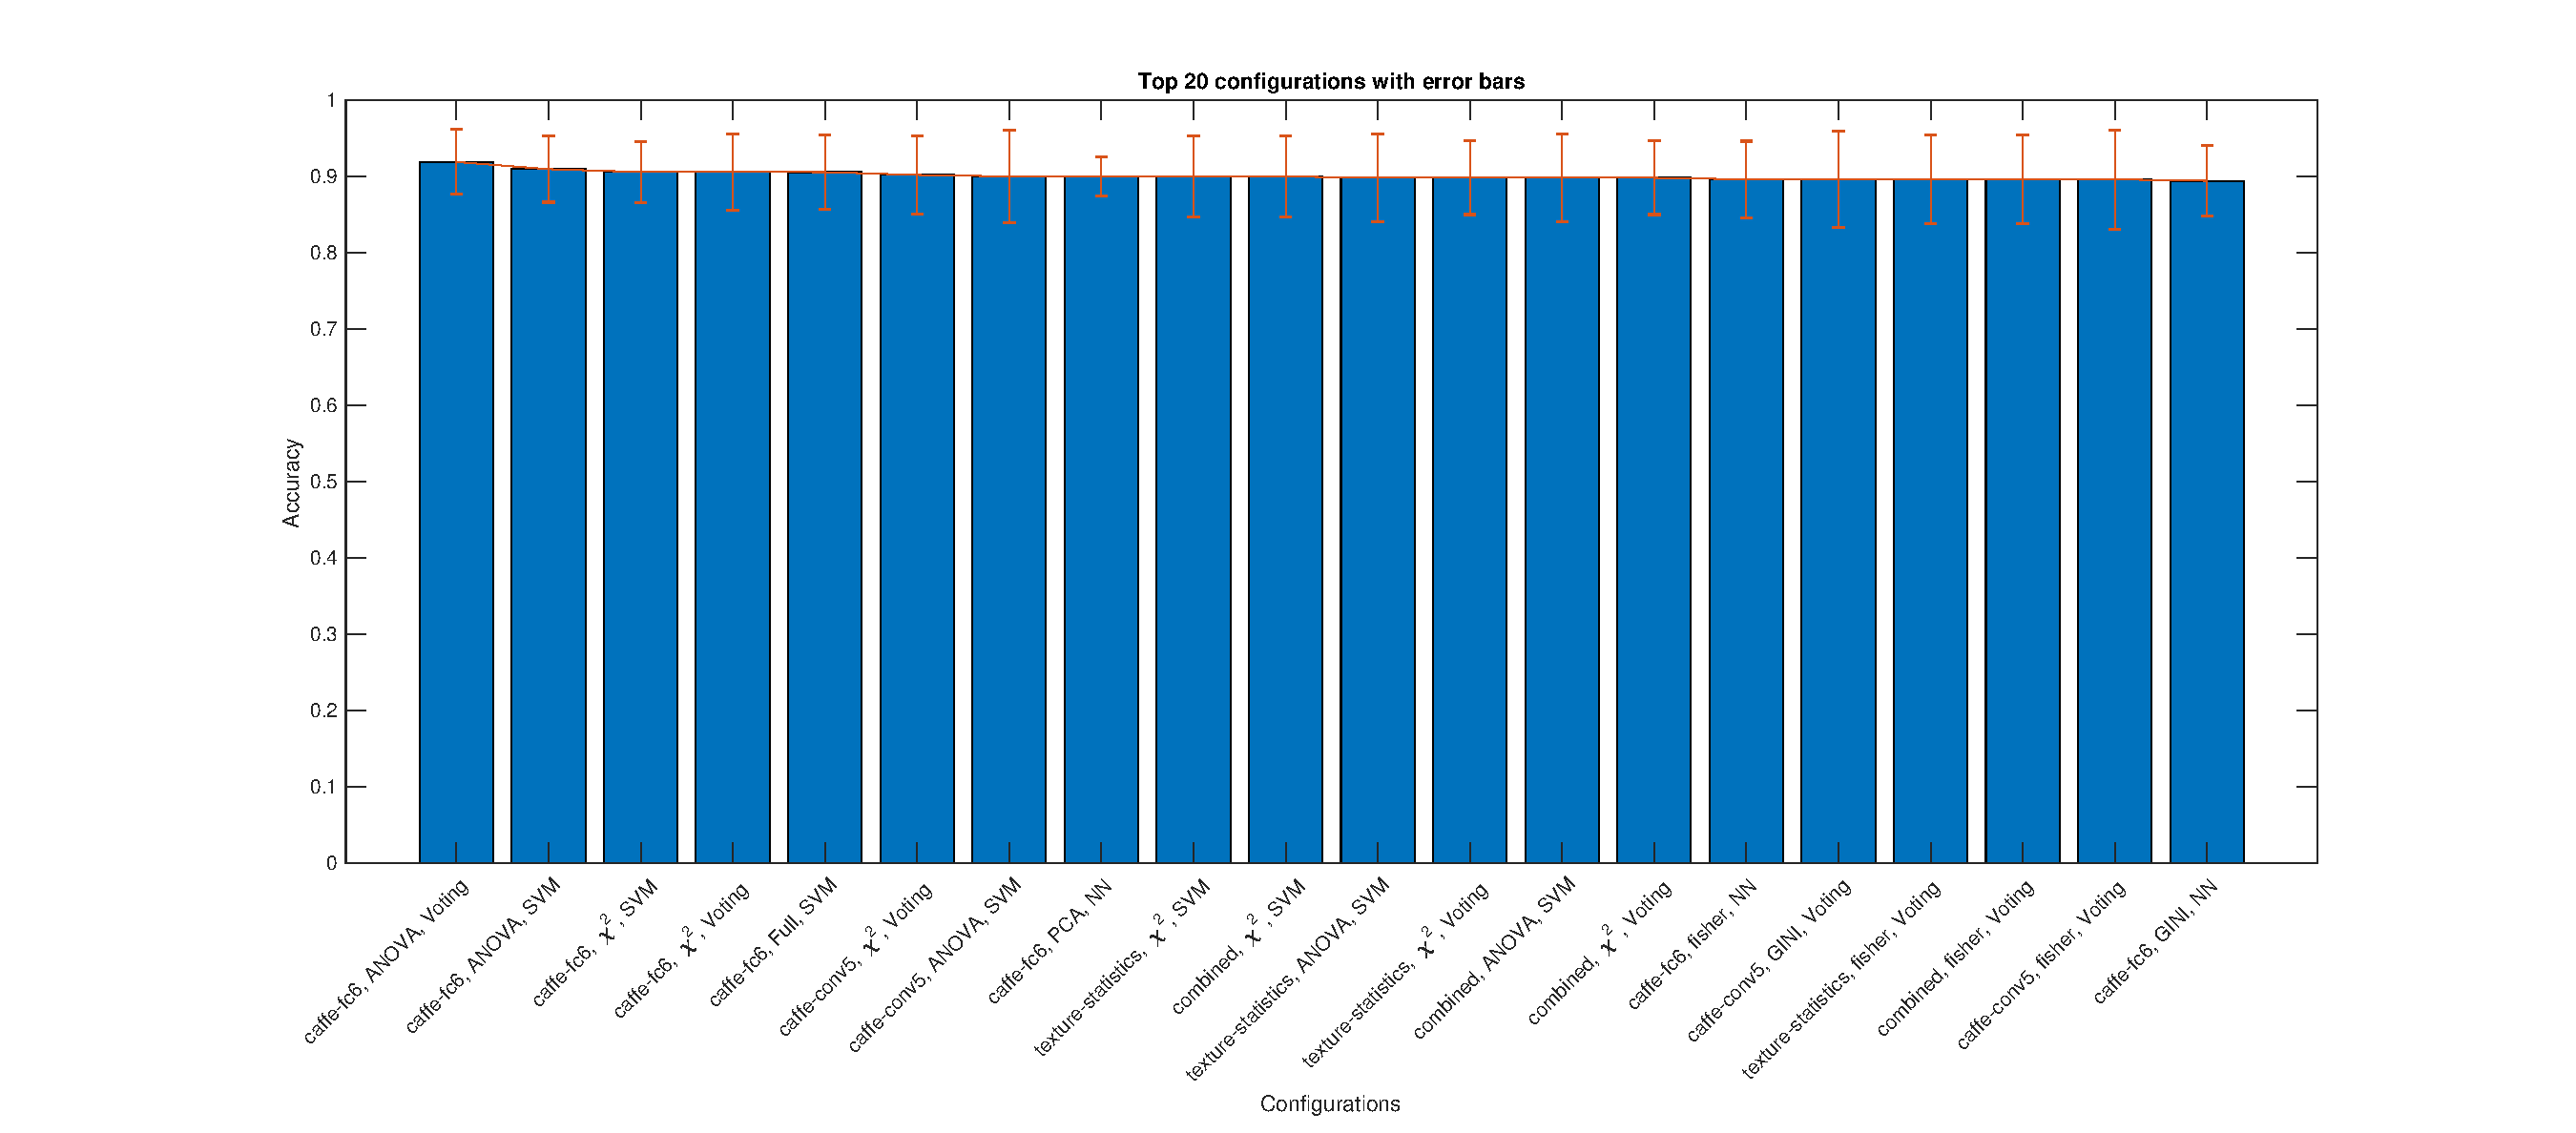
\includegraphics[scale=0.4]{img/best_matsc_error_bars_20.eps}
 \caption{Top 20 configurations of algorithms in Task 1 with error bars representing one standard deviation. There is no significant difference in the accuracies in the different configuations. Most of the feature extraction algorithms in the top 20 configurations are pre-trained CNNs (\textit{caffe-fc6} or \textit{caffe-conv5})}
 \label{fig:error_bars1}
 \end{centering}
\end{figure}

We can see from results in Table \ref{table:average_rank1} that caffe-fc6, $\chi^2$ and SVM are the best algorithms in the corresponding steps of feature extraction, dimensionality reduction and classification. However, caffe-fc6 has a larger margin with respect to the second best algorithm than $\chi^2$ and SVM in their respective steps. This indicates that caffe-fc6 is a good representation of the images for classification in Task 1.

\begin{table}[ht!]
\centering
\caption{Average rank of the algorithms in Task 1 with respect to feature extraction, dimensionality reduction and classification. The average rank of an algorithm quantifies it's position in the sorted list of configurations.}
\begin{tabular}{ |c|c| } 
 \hline
 \textbf{Feature extraction} & \textbf{Average rank} \\ 
 \hline
 caffe-fc6 & 47.82\\
 \hline
texture-statistics & 61.46\\
 \hline
combined& 64.46 \\
 \hline
caffe-conv5 & 72.39\\
 \hline
VBOW & 106.36\\
 \hline
 \hline
 \textbf{Dimensionality reduction} & \textbf{Average rank} \\ 
 \hline
 $\chi^2$ & 54.45\\
 \hline
fisher & 58.05\\
 \hline
PCA & 60.95 \\
 \hline
ANOVA & 61.80\\
 \hline
GINI & 66.10\\
 \hline
 Full & 66.55\\
 \hline
 \hline
 \textbf{Classification} & \textbf{Average rank} \\ 
 \hline
SVM & 54.57\\
 \hline
Voting & 60.8\\
 \hline
RF & 81.40 \\
 \hline
NN & 85.23\\
 \hline
 \end{tabular}
\label{table:average_rank1}
\end{table}

%--------------------------------------------------------------
\subsection{Task 2 - Longitudinal versus transverse cross-sectional views of dendrites} 
\label{Task2}
%--------------------------------------------------------------

Similar performance comparisons presented for Task 1 in Section \ref{Task1} were also completed for Task 2 (longitudinal vs. transverse cross-sectional views of dendrites).  A similar result was observed when feature extraction methods were evaluated, where caffe-fc6 represented micrographs well. 

Again, features extracted using pre-trained neural networks dominates Table \ref{tab:FE_Task2}. This result shows that the features extracted from the sixth, fully connected layer in the Caffe network (caffe-fc6) have meaningful and distinguishable characteristics in terms of microstructural images.  
%
Although the majority of the maximum classification accuracies used features extracted via caffe-fc6, even higher values for classification accuracy were obtained using texture statistics and caffe-conv5 with a a linear SVM classifier. Classification accuracies obtained via SVM-L varied based on the feature selection method used, however the overall classification accuracies were highest for this classifier with features computed from either texture statistics or caffe-conv5.  %These feature extraction methods, used in conjunction with various feature selection techniques and SVM-L could have resulted in higher classification accuracies due to.........
%
One major disadvantage of using texture statistics for feature extraction is that this method is a combination of multiple different feature detectors, and required prior knowledge of various techniques, that all perform differently depending on shape and texture of input data. 
%
The success of SVM as a classifier is subsequently discussed in additional detail.  

%---------------------------------------------------------------
%updated 06/10/16 - mrMR removed
\begin{table}[ht!]
\centering
\renewcommand{\arraystretch}{1}
\captionsetup{justification=centering}
\caption{Feature extraction methods and corresponding classification accuracies (in \%), that contributed to the maximum classification accuracy for each combination of feature selection and classification method tested for Task 2.}
\label{tab:FE_Task2}
\resizebox{\linewidth}{!}{
\begin{tabular}{|c|c|c|c|c|c|} \hline
	 & 	\multicolumn{5}{|c|}{\textbf{Classifier}} 									\\	\hline
\textbf{Feature }	&		&		&		&		&		\\	
\textbf{Selection}	&	\textbf{SVM-L}	&	\textbf{SVM-RBF}	&	\textbf{NN}	&	\textbf{RF}	&	\textbf{Voting}	\\	\hline
\multirow{2}{*}{\textbf{Full}}	&	texture-statistics 	&	\multirow{14}{*}{\textbf{caffe-fc6:} 95.74 $\pm$ 3.73}	&	\multirow{14}{*}{\textbf{caffe-fc6:} 94.49 $\pm$ 1.46}	&	\textbf{caffe-fc6} 	&	\multirow{14}{*}{\textbf{caffe-fc6:} 94.99 $\pm$ 2.38 }	\\	
	&	95.79 $\pm$ 3.94	&		&		&	87.88 $\pm$ 1.64	&		\\	
\multirow{2}{*}{\textbf{PCA}}	&	texture-statistics 	&		&		&	VBOW 	&		\\	
	&	96.84 $\pm$ 3.07	&		&		&	87.88 $\pm$ 2.95	&		\\	
\multirow{2}{*}{\textbf{ANOVA}}	&	texture-statistics 	&		&		&	\textbf{caffe-fc6} 	&		\\	
	&	97.37 $\pm$ 3.33	&		&		&	87.13 $\pm$ 1.64	&		\\	
\multirow{2}{*}{$\mathbf{{\chi}^2}$}	&	caffe-conv5 	&		&		&	caffe-conv5 	&		\\	
	&	96.78 $\pm$ 2.63	&		&		&	87.49 $\pm$ 15.69	&		\\	
\multirow{2}{*}{\textbf{fisher}}	&	caffe-conv5 	&		&		&	texture-statistics 	&		\\	
	&	97.84 $\pm$ 2.65	&		&		&	87.5 $\pm$ 8.25	&		\\	
\multirow{2}{*}{\textbf{GINI}}	&	caffe-conv5 	&		&		&	texture-statistics 	&		\\	
	&	97.31 $\pm$ 2.42	&		&		&	87.5 $\pm$ 8.25	&		\\	\hline

\end{tabular}}
\end{table}

%----------------------------------------------------------------------------------
Results from comparing feature extraction and classifier combinations indicate that in many cases feature selection did not improve calculated classification accuracies, as was seen in Task 1 results.  This is shown in Table \ref{tab:FS_Task2} by the majority of maximum classification accuracies computed using the full feature vector. 
%
When SVM-L was used for classification, feature selection methods improved results.  The feature selection method used with SVM-L that yielded the maximum classification accuracy depended on the feature representation obtained in the feature extraction step. 
%
The same classification accuracies were obtained for each feature selection method, for a given feature extraction and classifier combination. In addition, the features extracted from the fifth layer (convolutional) in the pre-trained neural network perform poorly with respect to the other extraction methodologies. This can be attributed to the fact that caffe-conv5 produces the feature representation with the highest dimensionality which is an order of magnitude greater than the second largest feature vector (caffe-fc6). Therefore, features extracted using caffe-conv5 are not robust (i.e. they have low accuracy with high standard deviation).  Being lower in the network hierarchy of the CNN also means that the features may not be tuned properly to the task, and therefore features provide a less accurate image representation than features computed via caffe-fc6.  
%----------------------------------------------------------------------------------
\begin{table}[ht!]
\centering
\renewcommand{\arraystretch}{1}
\captionsetup{justification=centering}
\caption{Feature selection methods, and corresponding classification accuracies (in \%), that contributed to the maximum classification accuracy for each combination of feature extraction and classification method tested for Task 2.}
\label{tab:FS_Task2}
\resizebox{\linewidth}{!}{
\begin{tabular}{|c|c|c|c|c|c|} \hline
	&	\multicolumn{4}{|c|}{\textbf{Classifier}} 							\\	\hline		
\textbf{Feature }	&		&		&		&		&		\\	
\textbf{Extraction}	&	\textbf{SVM-L}	&	\textbf{SVM-RBF}	&	\textbf{NN}	&	\textbf{RF}	&	\textbf{Voting}	\\	\hline
\multirow{2}{*}{\textbf{VBOW}}	&	ANOVA 	&	\textbf{Full}	&	\textbf{Full}	&	PCA 	&	\textbf{Full}	\\	
	&	96.32 $\pm$ 2.68	&	93.73 $\pm$ 3.96	&	 92.73 $\pm$ 3.91	&	87.88 $\pm$ 2.95	&	93.98 $\pm$ 3.09	\\	\hline
\multirow{2}{*}{\textbf{caffe-fc6}}	&	GINI 	&	\textbf{Full}	&	\textbf{Full}	&	\textbf{Full}	&	\textbf{Full}	\\	
	&	96.78 $\pm$ 2.63	&	95.74 $\pm$ 3.73	&	94.49 $\pm$ 1.46	&	87.88 $\pm$ 1.64	&	94.99 $\pm$ 2.38	\\	\hline
\multirow{2}{*}{\textbf{caffe-conv5}}	&	fisher 	&	\textbf{Full}	&	\textbf{Full}	&	${\chi}^2$	&	\textbf{Full}	\\	
	&	97.84 $\pm$ 2.65	&	84.46 $\pm$ 13.6	&	77.19 $\pm$ 14.62	&	 87.49 $\pm$ 15.69	&	78.45 $\pm$ 16.66	\\	\hline
\multirow{2}{*}{\textbf{texture-statistics}}	&	ANOVA 	&	\textbf{Full}	&	\textbf{Full}	&	fisher 	&	\textbf{Full}	\\	
	&	97.37 $\pm$ 3.33	&	93.23 $\pm$ 11.58	&	94.24 $\pm$ 5.03	&	87.5 $\pm$ 8.25	&	93.73 $\pm$ 11.09	\\	\hline
\multirow{2}{*}{\textbf{combined}}	&	ANOVA 	&	\textbf{Full}	&	\textbf{Full}	&	GINI 	&	\textbf{Full}	\\	
	&	97.37 $\pm$ 3.33	&	89.97 $\pm$ 9.08	&	87.97 $\pm$ 9.02	&	86.74 $\pm$ 2.98	&	84.46 $\pm$ 14.08	\\	\hline

\end{tabular}}
\end{table}

%-------------------------------------------------------------------------------------

Lastly, classification models were evaluated for each combination of feature extraction and feature selection with results presented in Table \ref{tab:Classifier_Task2}. SVM-L provided maximum accuracy with feature vectors calculated from the majority of feature extraction and selection methods.  Linear SVMs again yield the majority of maximum classification accuracies in this table (similar to Table \ref{tab:FE_Task1}, which shows that this classifier has the most distinguishable capacity among the different models tested. 

%For each feature extraction and selection combination, there is a single classifier that yielded the maximum classification accuracy (SVM-L). 
%The interesting trend in the results is that the classifiers are sensitive to the feature extraction techniques used. This trend may indicate that some classifiers are better adept at distinguishing the data depending on what feature extraction technique is implemented.

%Classification accuracies obtained via SVM-L varied based on the feature selection method used, however, overall the classification accuracies were highest for this classifier. 
%----------------------------------------------------------------
%-------------------------------------------------------------------------
%updated 06/10/16 -mrMR removed
\begin{table}[ht!]
\centering
\renewcommand{\arraystretch}{1}
\captionsetup{justification=centering}
\caption{Classification models that yielded the maximum classification accuracy (in \%) for each combination of feature extraction and feature selection method tested for Task 2.}
\label{tab:Classifier_Task2}
\resizebox{\linewidth}{!}{
\begin{tabular}{|c|c|c|c|c|c|} \hline
		&	\multicolumn{5}{|c|}{\textbf{Feature Extraction}} 									\\	\hline
\textbf{Feature }		&		&		&		&		&		\\	
\textbf{Selection}		&	\textbf{VBOW}	&	\textbf{caffe-fc6}	&	\textbf{caffe-conv5}	&	\textbf{texture-statistics}	&	\textbf{combined}	\\	\hline
\multirow{2}{*}{\textbf{Full}}		&	\textbf{SVM-L} 	&	SVM-RBF	&	\textbf{SVM-L} 	&	\textbf{SVM-L} 	&	\textbf{SVM-L} 	\\	
		&	95.26 $\pm$ 3.07	&	95.74 $\pm$ 3.73	&	88.57 $\pm$ 12.67	&	95.79 $\pm$ 3.94	&	95.79 $\pm$ 3.94	\\	\hline
\multirow{2}{*}{\textbf{PCA}}		&	\textbf{SVM-L} 	&	\textbf{SVM-L} 	&	\textbf{SVM-L} 	&	\textbf{SVM-L} 	&	\textbf{SVM-L} 	\\	
		&	94.21 $\pm$ 3.07	&	96.29 $\pm$ 3.56	&	96.29 $\pm$ 2.09	&	96.84  $\pm$ 3.07	&	96.84  $\pm$ 3.07	\\	\hline
\multirow{2}{*}{\textbf{ANOVA}}		&	\textbf{SVM-L} 	&	\textbf{SVM-L} 	&	\textbf{SVM-L} 	&	\textbf{SVM-L} 	&	\textbf{SVM-L} 	\\	
		&	96.32 $\pm$ 2.68	&	96.26 $\pm$ 3.19	&	91.9 $\pm$ 6.58	&	97.37 $\pm$ 3.33	&	97.37 $\pm$ 3.33	\\	\hline
\multirow{2}{*}{\textbf{${\chi}^2$}}		&	\textbf{SVM-L} 	&	\textbf{SVM-L} 	&	\textbf{SVM-L} 	&	\textbf{SVM-L} 	&	\textbf{SVM-L} 	\\	
		&	94.74 $\pm$ 3.33	&	96.26 $\pm$ 3.19	&	96.78 $\pm$ 2.63	&	96.32 $\pm$ 3.16	&	96.32 $\pm$ 3.16	\\	\hline
\multirow{2}{*}{\textbf{fisher}}		&	\textbf{SVM-L} 	&	SVM-RBF 	&	\textbf{SVM-L} 	&	\textbf{SVM-L} 	&	\textbf{SVM-L} 	\\	
		&	94.15 $\pm$ 1.03	&	95.74 $\pm$ 3.73	&	97.84 $\pm$ 2.65	&	96.29 $\pm$ 2.67	&	96.29 $\pm$ 2.67	\\	\hline
\multirow{2}{*}{\textbf{GINI}}		&	Voting 	&	\textbf{SVM-L} 	&	\textbf{SVM-L} 	&	\textbf{SVM-L} 	&	\textbf{SVM-L} 	\\	
		&	93.98 $\pm$ 3.09	&	96.78 $\pm$ 2.63	&	97.31 $\pm$ 2.42	&	96.84 $\pm$ 3.07	&	96.84 $\pm$ 3.07	\\	\hline

\end{tabular}}
\end{table}

%-------------------------------------------------------------------------------------

Results presented here demonstrate that certain combinations of methods (feature extraction, selection and classification) yield higher classification accuracies than others.  
%Table \ref{tab:summary} summarizes key results from testing multiple feature extraction, selection and classification methods.  
The sixth fully connected layer in the Caffe network proved to represent micrograph data well for both tasks.  The feature selection method for Task 1 depended on which classification model was used.  For Task 2, the full feature vector yielded the maximum classification accuracies, thus feature selection did not appear to improve classification results for most classifiers tested.  For classification models tested, linear SVM yielded the best results (highest accuracy) for both Tasks 1 and 2.  

%-------------------------------------------------------

Similar to Fig. \ref{fig:error_bars1} for Task 1, we plot the top 20 configurations with respect to the mean of the classification accuracies for Task 2 in Fig. \ref{fig:error_bars2}. Again, we observe the trend that there is no one clear \textit{best} configuration. We again show the average rankings of the algorithms in their respective steps of feature extraction, dimensionality reduction and classification in Table \ref{table:average_rank2}. 
\begin{figure}
  \begin{centering}
 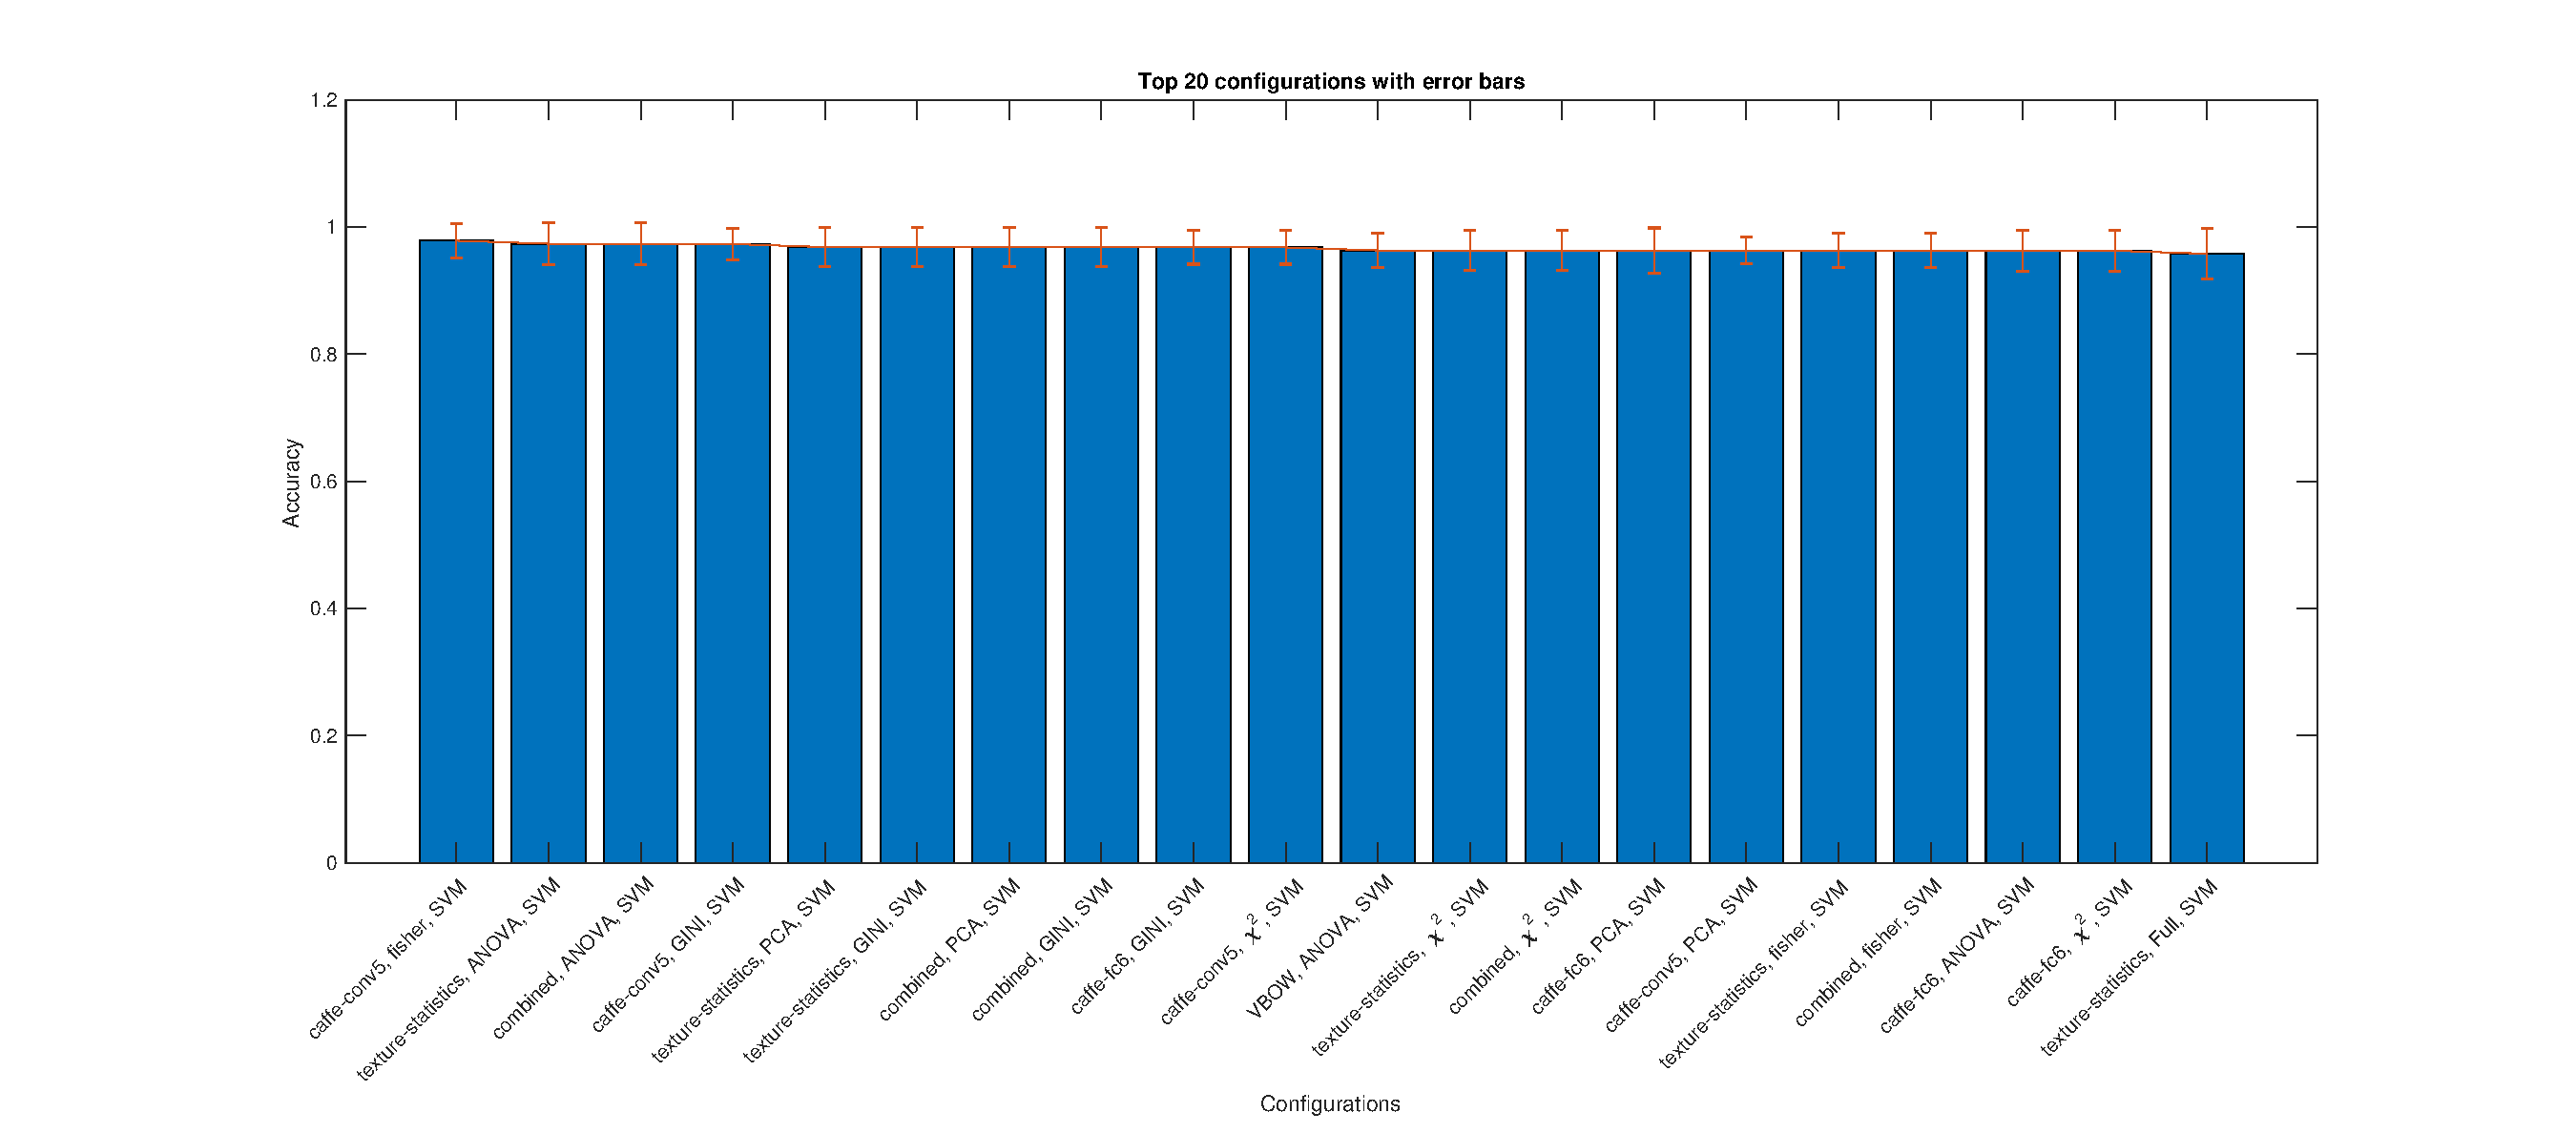
\includegraphics[scale=0.4]{img/best_trans_long_error_bars_20.eps}
 \caption{Top 20 configurations of algorithms in Task 2 with error bars representing one standard deviation. There is no significant difference in the accuracies in the different configuations. Most of the feature extraction algorithms in the top 20 configurations are pre-trained CNNs (\textit{caffe-fc6} or \textit{caffe-conv5})}
 \label{fig:error_bars2}
 \end{centering}
\end{figure}

From the results in Table \ref{table:average_rank2}, we observe that caffe-fc6, PCA and SVM are the highest ranked algorithms. We also note that in this case, the difference in rank between SVM and the next best classification algorithm (NN) is much greater than the corresponding differences in feature extraction and dimensionality reduction. This indicates that the SVM classification algorithm provides superior performance with respect to this task.

\begin{table}[ht!]
\centering
\caption{Average rank of the algorithms in Task 2 with respect to feature extraction, dimensionality reduction and classification. The average rank of an algorithm quantifies it's position in the sorted list of configurations.}
\begin{tabular}{ |c|c| } 
 \hline
 \textbf{Feature extraction} & \textbf{Average rank} \\ 
 \hline
 caffe-fc6 & 47.64\\
 \hline
texture-statistics & 58.64\\
 \hline
VBOW & 70.5 \\
 \hline
combined & 81.82\\
 \hline
caffe-conv5 & 93.89\\
 \hline
 \hline
 \textbf{Dimensionality reduction} & \textbf{Average rank} \\ 
 \hline
 PCA & 54.45\\
 \hline
$\chi^2$ & 58.05\\
\hline
ANOVA & 61.80\\
 \hline
GINI & 66.10\\
 \hline
 fisher & 66.55\\ 
 \hline
Full & 69.6 \\
 \hline
 \hline
 \textbf{Classification} & \textbf{Average rank} \\ 
 \hline
SVM & 31.22\\
 \hline
NN & 71.6\\
 \hline
Voting & 75.20 \\
 \hline
RF & 103.97\\
 \hline
 \end{tabular}
\label{table:average_rank2}
\end{table}


\section{Limitations}
\label{limitations}

In this work, pre-trained CNN's were used \cite{Krizhevsky2012}.  Training a convolutional neural network on the small amount of image data provided in Data Sets 1 and 2 (528 and 188 images, respectively) could prove difficult and potentially provide poor results in comparison to the results reported here. The reason for this is that deep neural networks require large image data sets for training because of their capacity to learn complex functions and are therefore prone to overfitting.  The CNN used in this work was previously trained on millions of natural images, allowing for the model to generalize well to new data instances. Even though the original dataset that the neural network was trained on primarily consisted of natural images, we can see (from high classification accuracies) that the features extracted on micrographs provide meaningful representations.

There are an infinite number of potential material microstructures in the realm of materials science.  Micrographs are two-dimensional images that represent a small sample of a three-dimensional microstructure, where `microstructure' refers to material structure on a nanometer to centimeter length scale.  Microstructures are formed from thermodynamic and kinetic processes, and depend on the crystal structure (atomic arrangement) of constituent elements.  Although the elements on the periodic table are fixed, there are numerous combinations of these elements that can be processed and studied. 

Let's first consider a material with a specific chemistry. There are various processes (annealing, quenching, cold working, etc.) that could yield a variety of microstructures.  Additionally, the processed sample could be sectioned in different ways (transverse versus longitudinal, for example), again impacting the microstructure visible for subsequent analysis.  There are also multiple imaging techniques available over a broad range of length scales (nanometer to centimeter).  Images generated from different techniques have different contrast, brightness, and ranges of grayscale intensities or RGB levels.  Expand this thought process to consider all possible material systems that can be generated from known elements with numerous imaging techniques (light optical microscopy, scanning electron microscopy, transmission electron microscopy, etc.).  The possible microstructures we can analyze in the form of image data seems endless.  

Therefore, the variety in micrographs used for materials characterization is vast, which is why expert knowledge and experience is relied on for such tasks as recognition, interpretation, and characterization.  Training an algorithm to perform such classification/characterization tasks on diverse micrograph data sets is a challenge not only in organizing a data set for training, validation, and testing, but in obtaining reasonably good classification results (greater than random).  The limitation presented here, is in the inherent variability of micrograph data, which could make classification tasks challenging, particularly if only a small data set is available for training and testing.  

%----------------------------------------------------------------------------------
\section{Conclusions}
\label{conclusions}

Computer vision and machine learning methods were successfully applied to the challenge of recognizing specific microstructural features of interest (e.g. dendrites) with varying magnifications, chemistries, and orientations.
%
Two binary classification tasks were performed: classification between micrographs with and without dendrites (Task 1), and classification between longitudinal and transverse cross-sectional views of dendrites (Task 2).  Data sets for Task 1 and Task 2 were 528 and 188 total images respectively. We are able to distinguish between microstructural images in terms of the presence of dendrites. A further refinement of the images can also be performed amongst the dendritic micrographs with respect to their cross-section. %The relationship between the two tasks is clearly shown here.
%
\\
Feature extraction and dimensionality reduction techniques were utilized in order to represent micrographs in the form of feature vectors.  Classification was then performed using support vector machines (linear and non-linear), voting, nearest neighbor, and random forest models.
%
For each model, classification accuracy was calculated for full and reduced feature vectors, for each feature extraction and selection method tested. 
\\

Results demonstrated that pre-trained neural networks represented micrographs well, and required no previous knowledge of the nature of shapes or object within the images. Furthermore, when pre-trained neural networks were used in feature extraction the highest classification accuracies for the majority of classifier and feature selection methods tested were achieved. Thus pre-trained neural networks generalize well. 
%
Maximum classification accuracies of 91.85 $\pm$ 4.25\% and 97.37$\pm$ 3.33\% were obtained for Tasks 1 and 2 respectively. 
%
While computer vision and machine learning methods have previously been applied to microstructure image data \cite{DeCost2015, Impoco2015, XuH2015, Bostanabad2016, Taffese2015}, pre-trained deep neural networks have not yet been explored for this particular application, but have proven successful in other image recognition tasks \cite{Guo2016}.  \\

%
Recognition of microstructural features traditionally requires expert knowledge of the particular material system under consideration.  The image-driven machine learning approach to micrograph classification presented here challenges this paradigm. 

This chapter of the thesis shows how we can use exhaustive grid search based methods to find the best configuration of algorithms and hyperparameters for characterizing microstructures. This method in addition to more methods of hyperparameter optimization like random search, Bayesian optimization and other global optimization methods maybe used to minimize the error from classification tasks in material science and other domains. In the next chapter of the thesis, we observe how we can reduce the classification error by reducing imbalance in the dataset.

%----------------------------------------------------------------------------------
\section{Future Work}
\label{future_work}

Neural networks are a promising feature extraction method for micrograph representation that could be further developed for application in more sophisticated characterization techniques, thereby eliminating the requirement of expert knowledge for recognition, interpretation, and characterization of microstructrural image data.  
%
Future work related to the exploratory study presented here, could involve application of pre-trained CNN's to more diverse micrograph data sets, or higher-level characterization tasks, such as average grain size measurement or calculating area fraction of a second phase.  
Furthermore, we would also like to incorporate deep learning algorithms on larger and more diverse micrograph classification tasks.
%----------------------------------------------------------------------------------
\section*{Acknowledgments}
\label{acknowledgments}
This work was is supported by the NSF under Grant \#1056704 through the Metals and Metallic Nanostructures Program of the Division of Materials Research, and Grant \#1302231 through the Information Integration and Informatics Program of the Division of Information and Intelligent Systems.   
%
The authors wish to acknowledge Mr. Jesse Werden and Dr. Jie Mao for some of the image data used in this work. 
%
Additionally, the authors thank the reviewers for providing thoughtful and thorough comments that contributed to the quality and clarity of the manuscript. 

\chapter{BLOOD VESSEL CHARACTERIZATION USING VIRTUAL 3D MODELS AND CONVOLUTIONAL NEURAL NETWORKS IN FLUORESCENCE MICROSCOPY}
\label{chap:automated}

\let\thefootnote\relax\footnotetext{
This chapter previously appeared as:
A. Chowdhury, D.~V. Dylov., Q. Li, M. MacDonald, D.~E. Meyer, M. Marino and A. Santamaria-Pang, "Blood vessel characterization using virtual 3D models and convolutional neural networks in fluorescence microscopy" \emph{IEEE International Symposium on Biomedical Imaging}, pp. 629-632, 2017}

%%% INTRODUCTION
\section{Introduction}

Characterizing the morphology of vasculature in digital pathology is an important step in defining the microenvironment within brain tissue samples. In particular, understanding the geometry of vessel configuration and its changes during a disease may provide deeper insight into the progression of neuropathological degenerative diseases such as Alzheimer?s disease. Images acquired using 20x object from immunofluorescent (IF) stained 6 um tissue sections with collagen IV antibody are used in this work.  We attempt to characterize three different types of blood vessel morphologies which are found in relative abundance in our image data set. They are singular blood vessels with no visible lumen, singular blood vessels with a distinct lumen and blood vessels appearing as a pair; which we have named RoundLumen-, RoundLumen+, and Twins correspondingly.
In this work, we show that it is possible to characterize blood vessels using convolutional neural networks (CNN) as opposed to traditional image processing techniques which involve segmentation and hand-crafted feature extraction. Instead, here we use pre-trained CNN to extract features from the images. This technique of ?deep transfer learning? is compared to the visual bag of words (VBW) method for feature extraction \cite{yang2007evaluating}. We conclude from the results that the features from pre-trained CNN are able to distinguish the morphologies of blood vessels better than the standard VBW method. 
Additionally, our work also shows that the construction of 3 dimensional (3D) virtual models of vasculature using parametric methods is a promising tool for dealing with infrequent scenarios in vascular analysis of brain tissue section. Acquisition of natural training samples is a time consuming and labor intensive process. Deep learning requires abundant training data for tuning the large number of parameters of the various inherent models. If a certain class is imbalanced then the classification models could become prone to biased outcomes. The construction of 3D parametric models, presented here tackles these issues and creates a balanced high-fidelity classification model. 
In this study, we built a basic 3D vasculature model using our prior knowledge of blood vessel geometry, as guided by a pathologist. The 3D vasculature was repeatedly sliced at various angles and orientations to obtain 2D samples for training the machine learning model, thereby mimicking the physical sectioning of tissue during sample preparation for microscopy. In addition, a filtering technique was then used to fine-tune the virtual data to reflect the variability present in the naturally acquired samples. We train three models based on: virtual data, natural data and a mixture of both. The models are then tested on a reserved, independent portion of the naturally occurring data, with a hierarchical classification being performed to demonstrate a proof of concept. 
The first classification task involves distinguishing between singular blood vessels (RoundLumen) and pair of blood vessels (Twins). The second task of finer granularity is the classification between RoundLumen- and RoundLumen+. We report various metrics for both the classification tasks and observe that the artificial data improves upon the model trained from only the natural data.
As far as we know, this is the first attempt to model vasculature using parametric 3D geometric methods exclusively. Statistical 2D and 3D shape models have been used extensively in medical image segmentation as detailed in \cite{heimann2009statistical}. However, these models use the training samples to statistically find a model of the object of interest. We do not generate virtual 2D models because we believe that we can obtain more variability in the training data by sectioning from the 3D models. Additionally, the 3D models may be extended to various other modalities in medical imaging. 

%%% Data
\section{Data}

This section provides a detailed explanation of the different morphologies of blood vessels that are explored in this study. The first subsection is a description of the natural data curated from actual postmortem human tissue samples. The second subsection involves the description of the virtual 3D model of blood vessels which are used for generating samples for training the convolutional neural networks.

\subsection{Natural data}
FFPE Postmortem brain tissue samples from ten subjects with neurological disorders underwent sequential IF-multiplexing and fluorescent imaging. For each subject, approximately 25 images were acquired.   This involves a cycling process of tissue section staining with 2-3 dye-labeled antibodies, imaging, dye inactivation and repeated staining with a new set of dye-labeled antibodies. Images underwent illumination correction, registration, stitching and auto-fluorescence subtraction. Collagen IV was used as a marker to detect all blood vessels. An image overlay is shown in Fig. \ref{morphologies}.

\begin{figure}[H]
\centering
\includegraphics[width=1.0\textwidth]{img/morphologies}
\caption{Depiction of the different morphologies in the natural data with respect to a multichannel image, overlaid with different protein markers. The three types of morphologies analyzed in this study is represented on the right.}
\label{fig:morphologies}
\end{figure}

The number of instances of the three different types of morphologies are depicted in Table \ref{table:classes}.
\begin{table}
\label{table:classes}
\caption{Distribution of vascular morphologies}
\centering
\begin{tabular}{ | c | c |} 
\hline
\textit{RoundLumen-} & 689 \\ 
\hline
\textit{Roundlumen+} & 3427 \\ 
\hline
\textit{Twins} & 266 \\ 
\hline
Total & 4382 \\ 
\hline
\end{tabular}
\end{table}

\subsection{Virtual data}
The construction of the artificial model starts with defining a set of control points in three dimensional Cartesian coordinates. The control points reflect the basic structure that the blood vessel is supposed to represent. This is followed by interpolating between the points using a 3D cubic spline interpolator. This forms the skeleton or the center line that represents the center or the lumen of the blood vessel and is shown in Fig. 2(a). The 3D volume of the blood vessel is constructed after this step. We first define a number of parameters; the inner radius of the blood vessel (r); the outer radius (R). The number of sampling points along the spline (N); the number of sampling points in the radial direction (Nr). At each sampling point; we define a circular disk along the z-axis; by randomly perturbing the values of r and R. We also define an intensity model for the blood vessels depicted in Eq. \ref{eq:1}. From the natural images, it seems that the intensity is high in the periphery of the blood vessel and decays towards the lumen and as we move away from the periphery. We model this using an exponential decay in the following form:

\begin{equation}
I(d) = I_{max} \exp(- \alpha |r\prime - d|)
\label{eq:1}
\end{equation}


where, $I_{max}$  is the maximum intensity, is the calibration coefficient (in mm-1 units), $r\prime=(R+r)/2.$ $d$ is the distance from the center of the lumen. At each point on the disc, we define the voxel density as a normal distribution with mean $I(d)$ and standard deviation 0.01. This is followed by formulating the rotation matrix by calculating the angle between the tangent to the spline at that sampling point and the z-axis. The points corresponding to each point on the disc are therefore mapped or rotated along the curve by multiplying the coordinates with the rotation matrix. An example of this rotation is depicted in Fig. \ref{fig:3D_model}(b). We then discretize the coordinates such that we obtain an actual 3D image in the form of an array. This is depicted in Fig. \ref{fig:3D_model}(c). The intensity values are normalized and assigned to the corresponding discretized points in the 3-dimensional array. The volume rendered version of the 3D image is depicted in Fig. \ref{fig:3D_model}(d). Therefore, by changing the parameters of the model we can build several different 3D images and slice it at various angles to mimic the natural tissue cross sections at various depths and angles. Some examples the various models are depicted in Fig. \ref{fig:slicer}.

\begin{figure}[H]
\centering
\includegraphics[width=1.0\textwidth]{img/3D_model}
\caption{Development of the 3D virtual model}
\label{fig:3D_model}
\end{figure}

\begin{figure}[H]
\centering
\includegraphics[width=1.0\textwidth]{img/slicer}
\caption{3D virtual models and their corresponding projections along different planes of view (a) Linear model of RoundLumen- (b) Linear model of RoundLumen+ (c) Non-linear model of RoundLumen+ (d) Non-linear model of Twins}
\label{fig:slicer}
\end{figure}

The process of construction of the different types of morphologies in blood vessels is the same as that explained above. Fig.  \ref{fig:slicer}(a) is a blood vessel with a no lumen (RoundLumen-) and a linear skeleton. The control points are chosen such that they lie on the major diagonal of the unit cube; i.e. on the line x=y=z in Cartesian coordinates.  Figures  \ref{fig:slicer}(b) and  \ref{fig:slicer}(c) are blood vessel with a single lumen having linear and non-linear structures respectively. Fig.  \ref{fig:slicer}(d) is a model of a Twin. As we can see from the cross-sectional views, we obtain different types of morphologies that are similar to actual morphologies in the natural images. A very simple way of creating these multi-vessel structures is by perturbing or shifting the sampling points of the skeleton along a random direction. For example; to come up with a model of RoundLumen-, we simply set the inner radius r to 0. As shown in Fig. 3; the different morphologies that commonly occur naturally can be generated. As explained in the introduction; this serves as a viable alternative to using natural data for training convolutional networks.

\section{Methods}

A convolutional neural network is a type of artificial neural network in which are inspired by the organization of the 
animal visual cortex. CNNs consist of multiple neuron collections which process portions of the input image called receptive fields. The outputs are then tiled so that the input regions overlap and this in turn produces a better representation of the original image. This is what makes CNNs translation invariant. 
The CNN is made up of four types of layers: the input layer, the convolutional layer, the non-linear layer, the pooling layer; and the fully connected layer. The input layer is where the networks accept the images.  The images consist of raw pixel values depicted by width, height and the number of channels.  The convolutional layer will compute the output of the neurons that are connected to local regions in the input, each computing a dot product between their weights and a receptive field. The non-linear layer is the activation function responsible for introducing the non-linearity in the model. The various types of non-linear functions include the sigmoid, the tanh, and the rectified linear unit. The pooling layer performs a down sampling operation. The high-level reasoning in the neural network is done by fully connected layers.  Their activations can be performed by simple matrix multiplication.
In this work, we use the pre-trained convolutional neural networks as a feature extractor. This network consists of weights trained on the ImageNet dataset. We extract the 6th layer in the network which is a 4096-dimensional vector as a representation of the image. This may be considered as a transfer learning model because we transfer the weights learnt from another domain to blood vessel recognition. We use a pre-trained neural network called AlexNet \cite{krizhevsky2012imagenet} to extract features from the data. 

We perform an experiment to show that pre-trained CNNs are efficient in representing the vascular morphology. The experiment is performed on the natural data where 33 \% of the data is held out as test data and the rest is used for training. Two models are developed. One of them uses the visual bag of words (VBW) \cite{yang2007evaluating} feature extraction method to extract the features; the other uses the AlexNet architecture to extract the features. A three-class classification (one vs rest) is performed using the logistic regression classifier. The accuracy, f1-score, precision and recall calculated on the same test data are reported for comparison.

\begin{table}[H]
\centering
\caption{Comparison of feature extraction methodologies}
\begin{tabular}{ | c | c | c | c | c |} 
\hline
Feature extractor  & Accuracy	& f1-score	 & Precision & Recall \\ 
\hline
\textit{AlexNet} & 91.92 & 91.93 & 91.98 & 91.92 \\ 
\hline
\textit{VBW} & 78.38	& 77.38 & 	76.71 & 78.38 \\
\hline
\end{tabular}
\label{table:FE}
\end{table}

The results in Table \ref{table:FE} show that pre-trained convolutional neural networks are a good choice for representation of vascular morphology.

\section{Experiments and results}
Features are extracted using the AlexNet architecture which is trained on the ImageNet \cite{deng2009imagenet} database. The weight parameters are used to extract the features in a feedforward manner. This is called transfer learning. 33 \% of the natural data is held out as test data. All the experiments are performed on this dataset for maintaining consistency in the results. 
A filtering technique is introduced to appropriately extract slices from the 3D volumes. This is done by obtaining the probabilities of the artificial data using a model trained on the natural training data. The probabilities of the corresponding images are then sorted and the images with the highest probabilities are selected. This is a way to boost the artificial model.  The filtered virtual data is then used to retrain the classifier. Examples of both the natural and artificial data are represented in the Fig. \ref{fig:slices}.

\begin{figure}[H]
\centering
\includegraphics[width=1.0\textwidth]{img/slices}
\caption{ Examples of vessel classes RoundLumen- (a/d), RoundLumen+ (b/e) and Twins (c/f) for natural (a/b/c) and virtual data (d/e/f)}
\label{fig:slices}
\end{figure}

A hierarchical classification is performed to first classify the single blood vessels from blood vessels that bundled in pairs i.e RoundLumen vs Twins. The second classification task involves distinguishing between RoundLumen- and RoundLumen+. We perform three different types of training to demonstrate our proposed methods. The first type of training is done with only the naturally occurring data. The second type of training data consists only of the artificial data that has been filtered by the natural model as explained before. Finally, the third type consists of both the artificial and natural training samples. We refer to this as Mixed. All the results are reported on the held out 33 \% of the natural data. The accuracy, f1-score, precision, recall and receiver operating characteristic (ROC), and precision-recall (PR) curves are reported in the following tables and figures for each of the two classification tasks. 

\begin{table}[H]
\label{table:results}
\centering
\caption{Results of binary classification between RoundLumen and Twin}
\begin{tabular}{ | c | c | c | c | c |} 
\hline
Data & Accuracy & f1-score & Precision & Recall \\ 
\hline
\textit{Artificial} & 92.81& 59.36	& 45.24 & \textbf{86.36} \\ 
\hline
\textit{Natural} & 96.34& 71.03& 68.42& 73.86 \\
\hline
\textit{Mixed} & \textbf{97.71} & \textbf{81.76} & \textbf{79.57} & 84.01 \\
\hline
\end{tabular}
\end{table}

\begin{figure}[H]
\centering
\includegraphics[width=1.0\textwidth]{img/results}
\caption{ROC curves for classification: (a) \textit{RoundLumen} and  \textit{Twins}  and (b) \textit{RoundLumen-} and \textit{RoundLumen+} .}
\label{fig:results}
\end{figure}


\begin{table}[H]
\label{table:results1}
\centering
\caption{Results of binary classification between \textit{RoundLumen-} and \textit{RoundLumen+}}
\begin{tabular}{ | c | c | c | c | c |} 
\hline
Data & Accuracy & f1-score & Precision & Recall \\ 
\hline
\textit{Artificial} & 98.38 & 99.02 & 99.38 & 98.67 \\ 
\hline
\textit{Natural} & 96.34& 71.03& 68.42& 73.86 \\
\hline
\textit{Mixed} & \textbf{98.60} &  \textbf{99.16} & \textbf{99.29} & \textbf{99.03} \\
\hline
\end{tabular}
\end{table}

The ROC curves are calculated using the minority class in both the classification tasks, i.e. Twins for the first classification task and RoundLumen- for the second task.
From Table \ref{results}, we can see that the artificial data captures the differences between the two classes. It is also able to identify \textit{Twins}, which is the minority class in Task 1, from the high recall. Therefore, the results are boosted when we combine both the artificial and natural data. In addition, the ROC curves in Figure 6 confirms our hypothesis that virtual data may be used for building the models. The naturally trained model performs better than the virtual trained model. However, as we can see from the ROC curves, the model built from the mixed data improves the performance. Table \ref{results1} presents the corresponding results for the second classification task. In this case, we see that the virtual data performs better than the natural data and boosts the performance when trained on its own or in union with the natural data.

\section{Conclusions}
We have shown that the use of deep learning algorithms ?  trained with a mixture of virtual and natural data ?  results in a more accurate prediction of vasculature morphologies than the use of standard feature extraction methods (such as visual bag of words). The methodology of complementing natural data with synthetic samples holds potential for becoming a standard approach in deep learning with unbalanced datasets. In neuroscience, it could be applied to help elucidate the underlying mechanisms of common neurological degenerative diseases.
\chapter{A MACHINE LEARNING BASED APPROACH TO QUANTIFYING NOISE IN MEDICAL IMAGES}
\label{chap:SPIE1}

\let\thefootnote\relax\footnotetext{
Parts of this chapter previously appeared as:
A. Chowdhury, K.~S. Aggour, S.~M. Gustafson, B. Yener,
``A Machine Learning Approach to Quantifying Noise in Medical Images.''
\emph{Medical Imaging 2016: Digital Pathology},
vol. 9791, pp. 979110U, 2016.}

%%% INTRODUCTION
\section{Introduction}

This chapter is the first of the two works that focus on quantification of the components of the image classification pipeline. Here, we show how we can use a a machine learning based score to quantify the noise in the image sample itself. 
As advances in medical imaging technology are resulting in significant growth of biomedical image data, new techniques are needed to automate the process of identifying images of low quality. Automation is needed because it is very time consuming for a domain expert such as a medical practitioner or a biologist to manually separate good images from bad ones. While there are plenty of de-noising algorithms in the literature, their focus is on designing filters which are necessary but not sufficient for determining how useful an image is to a domain expert.
Thus a computational tool is needed to assign a score to each image based on its perceived quality. In this paper, we introduce a machine learning-based score and call it the \textit{Quality of Image (QoI)} score. The \textit{QoI} score is defined based on the probabilities of classification using the logistic regression classifier.
We test our technique on clinical image data obtained from cancerous tissue samples. We used 723 tissue samples that are stained by three different markers (abbreviated as CK15, pck26, E\_cad) leading to a total of 2,169 images. Our automated labeling is in agreement with the domain experts with an F1-score of 0.9044 on average. The results show a distribution of the \textit{QoI} score for each of the three markers that correspond to the actual quality of the images from the marker according to the pathologist who labelled the images based on their perceived quality.  We also quantify the quality of the markers and their differences based on the \textit{QoI} scores of each sample stained using that marker. 
Furthermore, we propose a data-driven method by which images maybe recovered based on the \textit{QoI} score and forwarded for further post-processing.

%%% Data
\section{Data}

The data we use is in the form of microscopic images. The colon cohort in this analysis was collected from the Clearview Cancer Institute of Huntsville Alabama from 1993 until 2002, with 747 patient tumor samples collected as formalin-fixed paraffin-embedded specimens. The median follow-up time of patients in this cohort is 4.1 years, with a maximum of over ten years. Stage 2 patients comprise 38 \% of this cohort, stage 1 and 2 combined are 65 \% of the total patients. We have stained and processed 747 CRC subjects described above on tissue microarrays for 63 target proteins of consequence to cancer biology and ancillary image processing and analysis. A full description of materials and methods was described recently in \cite{gerdes2013highly}.
The images in this work are stained with three different markers. The markers are Ecadherin (E\_cad), pan-Keratin (pck26) and Keratin15 (CK15). The three markers stain epithelial cells in the tissue. The raw dataset consists of 747 tissue samples and each tissue sample has four images from each marker; resulting in a total of 2,988 images.  723 images from the 747 samples were selected by the pathologist for this work which result in a total of 2169 images from all the 3 stains.
The images marked with E\_cad have the least amount of noise associated with them. Images stained with pck26 is more noisy than E\_cad, while CK15 is the noisiest among the 3 markers with respect to the presence of undesirable artifacts in the image. This difference in quality maybe observed from Fig. \ref{fig:example_images} from each of the 3 protein markers. We quantify the quality of  both images and markers using the \textit{QoI} score defined in this paper. 

\begin{figure}
    \centering
    \begin{subfigure}[b]{0.3\textwidth}
        \centering
        \includegraphics[width=\textwidth]{img/SPIE/ecad_example.eps}
        \caption{E\_cad}
        \label{fig:ecad_example}
    \end{subfigure}
    \hfill
    \begin{subfigure}[b]{0.3\textwidth}
        \centering
        \includegraphics[width=\textwidth]{img/SPIE/pck26_example.eps}
        \caption{pck26}
        \label{fig:pck26_example}
    \end{subfigure}
    \hfill
    \begin{subfigure}[b]{0.3\textwidth}
        \centering
        \includegraphics[width=\textwidth]{img/SPIE/CK15_example.eps}
        \caption{CK15}
        \label{fig:CK15_example}
    \end{subfigure}
    \caption{Examples of a single colon tumor tissue sample stained with three different markers. E\_cad is the least noisy with respect to undesirable artefacts, followed by pck26 and CK15 respectively.}
    \label{fig:example_images}
\end{figure}

\subsection{Feature extraction}

We quantify the information in the three markers (E\_cad, pck26, CK15) by texture features. Texture based features maybe used as a way to quantify the difference between images based on amount of signal or noise in an image, and be able to distinguish between images of the types shown in Fig. \ref{fig:example_images} .  These set of 13 features are based on gray-level intensity values, and texture information \cite{haralick1979statistical, haralick1973textural} in the images. 
Haralick features \cite{Haralick1973} are calculated using gray-level co-occurrence matrices (\textit{G$_{ij}$}, shown below) which are square matrices of size \textit{N$_g$} x \textit{N$_g$}, where \textit{N$_g$} is the number of gray levels in an image:
\\
\begin{equation}
%\[
G_{ij}=
  \begin{bmatrix}
    p(1,1) & p(1,2) & \cdots       & p(1,N_{g}) \\
    p(2,1) & p(2,2) &  \cdots      & p(2,N_{g}) \\
     \vdots &  \vdots &  \ddots    &  \vdots          \\
    p(N_{g},1)  & p(N_{g},2) & \cdots & p(N_{g},N_{g}) 
  \end{bmatrix}
%\]
\end{equation}
\\
Each matrix element, $ \ [i,j]\ $, is calculated by counting the number of times a pixel with value \textit{i} is adjacent to pixel with value \textit{j}.  When considering a square pixel image, there are four directions for which a gray-level co-occurrence matrix can be calculated: horizontal, vertical, left diagonal, and right diagonal.  Haralick texture statistics can be calculated based on the four gray-level co-occurrence matrices from each of these four directions. Haralick features thus describe the texture of an image. Fundamentally, texture is the arrangement of a certain feature or property, relative to the environment. In images, texture is the spatial distribution (arrangement) of gray-level variations in an image. Haralick features, computed from image gray-level co-occurrence matrices, capture texture patterns in an image. 

In addition to the features, labels are assigned to each image by domain experts based on the amount of noise in them. The label +1 is assigned if the image has some signal in it. This class is colloquially referred to as the \textit{good} class.  Images with a lot of noise in them where there is almost no signal are labelled as -1 or the \textit{bad} class.

\subsection{Data preprocessing}
The three markers (CK15, pck26, E\_cad) corresponding to each tissue sample are combined together to provide us with 723 x 3 = 2169 samples. We perform 5-fold cross validation on this data to compute the quality of image score and report the accuracy and F1-score on the validation data.
The data is highly imbalanced. The ratio of bad to good images is roughly 1 : 18. Therefore, it is important to try to redress this imbalance. We use the synthetic minority oversampling technique (SMOTE) \cite{chawla2002smote} on this data to perform oversampling.  In this data balancing technique, the minority class (\textit{bad}) is oversampled by introducing synthetic samples along the line joining any or all of the k minority class nearest neighbors. Here \textit{k} is set as 5. The number of neighbors from the \textit{k} - nearest neighbors are randomly chosen depending on the amount of oversampling needed.

Principal components analysis (PCA) \cite{wold1987principal} is performed to reduce the number of features from 13 such that it captures 95 \% of the information. This reduces the number of dimensions to 5.
PCA is a feature transformation technique that uses orthogonal transformation to convert a set of observations of correlated variables to linearly uncorrelated ones. These orthogonal components are called principal components. PCA can be thought of as a transformation that reveals the structure of the data in a way that best explains the variance in the data. The drawback of this technique is that the features obtained after reduction are linear combinations of the original feature variables which occupy a different vector space than the original variables. 


\section{Methods and experiments}
In this section, we describe the methods that we used in our analysis of the images and also show the results that we achieved from the application of these methods on our data.

\subsection{Classification and analysis}
The features from all the 3 markers are combined to form a feature matrix of size 2169 x 5 (after dimensionality reduction using PCA). We combine the data together for two reasons. The first reason is that this provides more samples for training. The second reason is that we want to create a quantity that quantifies the score over all the markers and is not just trained on one marker. 
We used the logistic regression classification algorithm for performing classification. We choose logistic regression algorithm because it is a simple classification algorithm that can make binary decisions. In addition, the sigmoid function used in logistic regression, squashes the the output of the linear function between 0 and 1. This value can be directly interpeted as a probability. This is exactly what we define as the \textit{QoI} score in Eq. \ref{eq:1} defined in the next section.
The F1-score for classification using the feature matrix on the binary classification problem is 0.9044 ($\pm$  0.03 standard deviation). We use the F1-score instead of accuracy as the classification metric because of the imbalance in the dataset.

\subsection{Quality of image score}
The \textit{Quality of Image (QoI)} score is defined as the probability that an image is from the \textit{good} class. It is given by Eq. \ref{eq:1}.
\begin{equation}
\begin{gathered} 
S_i \ =  \ p_{i1} 
\end{gathered}
\label{eq:1}
\end{equation}
A high value of the probability indicates that the image has high quality and must be used for further analysis. A low value of the probability denotes that the image belongs to the \textit{bad} class and it can be discarded. An intermediate value of the probability is interesting because it denotes there is some signal in the image and that it may or may not be used for analysis. We denote such an image to be \textit{ugly} which is neither \textit{good} nor \textit{bad}.
 The three sample images in the following figure show examples \textit{good}, \textit{bad} and \textit{ugly} classes according to the QoI score. 

\begin{figure} [ht!]
    \centering
    \begin{subfigure}[b]{0.3\textwidth}
        \centering
        \includegraphics[width=\textwidth]{img/SPIE/E_cad_AFRemoved_260143_9945.eps}
        \caption{A \textit{good} image from E\_cad marker with a \textit{QoI} of 0.9945}
        \label{fig:good}
    \end{subfigure}
    \hfill
    \begin{subfigure}[b]{0.3\textwidth}
        \centering
        \includegraphics[width=\textwidth]{img/SPIE/CK15_AFRemoved_269_084_0077.eps}
        \caption{A \textit{bad} image from CK15 marker with a \textit{QoI} of 0.0077}
        \label{fig:bad}
    \end{subfigure}
    \hfill
    \begin{subfigure}[b]{0.3\textwidth}
        \centering
        \includegraphics[width=\textwidth]{img/SPIE/pck26_AFRemoved_260_084_5262.eps}
        \caption{A \textit{ugly} image from pck26 marker with a \textit{QoI} of 0.5262}
        \label{fig:ugly}
    \end{subfigure}
    \caption{Examples of \textit{good}, \textit{bad} and \textit{ugly} images based on the \textit{QoI} score.}
    \label{fig:gbu}
\end{figure}

Fig. \ref{fig:gbu} shows examples of the images from the test data with their corresponding \textit{QoI} scores. Fig \ref{fig:good} stained using the E\_cad marker shows an image with a high \textit{QoI} score. This image is clearly a \textit{good} image as the tissue is easily observable and is not occluded. This image must be used for further analysis. Fig. \ref{fig:bad} is an example of an image with a low \textit{QoI} from the CK15 marker. This is image has literally no tissue and has regions of occlusions. This image should definitely be discarded. The third image in Fig. \ref{fig:ugly} from the pck26 marker, has some signal in it in terms of tissue but is also plagued with some noise. This is an example of what we call an \textit{ugly} image and this sample may or may not be used in further analyses.

\subsection{Results and discussion}
We plot the distribution of \textit{QoI} scores in Fig. \ref{fig:distribution}. Figs. \ref{fig:all_probs}, \ref{fig:ecad_probs}, \ref{fig:ck15_probs}, \ref{fig:pck26_probs} correspond to the distribution of the images from all markers, E\_cad, CK15 and pck26 respectively. 

\begin{figure}[ht!]
\centering
\begin{subfigure}{.5\textwidth}
  \centering
  \includegraphics[scale=0.37]{img/SPIE/all_probs_smote_pca.eps}
  \caption{Distribution of scores on all the images}
  \label{fig:all_probs}
\end{subfigure}%
\begin{subfigure}{.5\textwidth}
  \centering
  \includegraphics[scale=0.37]{img/SPIE/E_cad_probs_smote_pca.eps}
  \caption{Distribution of scores from E\_cad marker.}
  \label{fig:ecad_probs}
\end{subfigure}
\begin{subfigure}{.5\textwidth}
  \centering
  \includegraphics[scale=0.37]{img/SPIE/CK15_probs_smote_pca.eps}
  \caption{Distribution of scores from CK15 marker.}
  \label{fig:ck15_probs}
\end{subfigure}%
\begin{subfigure}{.5\textwidth}
  \centering
  \includegraphics[scale=0.37]{img/SPIE/pck26_probs_smote_pca.eps}
  \caption{Distribution of scores from pck26 marker}
  \label{fig:pck26_probs}
\end{subfigure}
\caption{Distribution of \textit{QoI} scores on the images. According to the pathologist, the perceived quality of the images from the E\_cad and pck26 marker is good and the images from the CK15 marker has low signal and high noise in general.  This is reflected in the distribution of these markers}
\label{fig:distribution}
\end{figure}

The pathologist who labelled the images as \textit{good} or \textit{bad} based on the perceived quality of the images claimed that the images from the CK15 marker has more noise than images from E\_cad and \textit{pck26}. This is exactly what we quantify using the \textit{QoI} score. The ratios of \textit{good} to \textit{bad} images for E\_cad, CK15 and pck26 are approximately 19:1, 19:1 and 17:1 respectively for the three markers. The difference in quality of the images are not captured by the distribution of the labels themselves. The distributions of the scores of the three markers in Fig. \ref{fig:distribution} clearly quantify this difference. We can see from Figs. \ref{fig:ecad_probs} and \ref{fig:pck26_probs} that the \textit{QoI} scores are skewed towards higher values close to one. On the other hand Fig. \ref{fig:ck15_probs} shows that there are a large number of images that maybe denoted as \textit{ugly}. The average values of the probabilities over all the images in a marker can be used to quantify the quality of the marker itself. In fact, the average values of the probabilities over all images in E\_cad, CK15 and pck26 are 0.85, 0.54 and 0.82 respectively.  Therefore, the quality of the markers E\_cad and pck26 is better than that of CK15. We divide the range of the scores into 3 equally spaced regions to demonstrate the difference between the three markers in more detail. The three regions are denoted as \textit{good} with a score range of 0.67 to 1, \textit{bad} with a range of 0 to 0.33 and \textit{ugly} with a range of 0.33 to 0.67. These values are chosen to demonstrate the differences between the markers. We discuss methods to select these thresholds later.

\begin{table}[ht!]
\centering
\caption{Percentage of the number of images that fall in the \textit{good}(0.67- 1), \textit{bad} (0 - 0.33) and \textit{ugly} (0.33 - 0.67)regions of the QoI score with respect to the 3 markers. The percentage values clearly quantify the claim that E\_cad is the least noisy followed by pck26 and CK15.}
\begin{tabular}{ |c|c|c|c|} 
 \hline
\textbf{Marker} & \textbf{good} (\%)& \textbf{bad} (\%) & \textbf{ugly} (\%)\\ 
 \hline
E\_cad & 43.14 & 16.33 & 10.54\\
 \hline
pck26 & 40.15 & 19.52 & 18.61\\
 \hline
CK15 & 16.71 & 64.14 & 70.85\\
 \hline
 \end{tabular}
\label{table:scores}
\end{table}


Let's focus on the region between the scores of 0.33 and 0.67, which we may denote as the \textit{ugly} region of the \textit{QoI} score in Table \ref{table:scores}. The percentage of images from E\_cad, pck26 and CK15 that fall in this region are 16.33 \%, 19.52 \% and 64.14 \% respectively. These values also show that there are more contentious images  with respect to the \textit{QoI} score in CK15 than in E\_cad and pck26.
We also show  the distribution of the scores over all the images in the three markers in Fig. \ref{fig:all_probs}. The plot shows that most of the images have high quality. This is because images from E\_cad and pck26 which have high amounts of signal (according to the pathologist) account for two-thirds of the total data.
It is clear from the results that the \textit{QoI} score maybe used to quantify the amount of usable signal in the image.  The \textit{QoI} of an image sample provides an indication as to whether a particular sample may or may not be used in the analysis. 

There could be a number of different ways to use the \textit{QoI} scores usefully for performing analysis. In Table \ref{table:scores}, we selected the thresholds arbitrarily by dividing the range of the scores into 3 equally spaced regions - \textit{good}, \textit{bad} and \textit{ugly}.  A threshold maybe set on the QoI by the analyst and only those images above the threshold can be used for further analysis. Alternatively, a data-driven approach maybe used to leverage the \textit{QoI} score for performing further analysis. For example, the next step of the process maybe to classify the images into different grades of cancer.
In this step the \textit{QoI} score can be obtained for the dataset in question. The classification maybe started with a sample of images that have \textit{QoI} above a certain threshold. Then images are added to the training in batches based on the \textit{QoI} scores in a sequential manner. This procedure maybe repeated until the accuracy on the held out test set plateaus or decreases. This threshold could be used as the cutoff \textit{QoI} score to threshold the images for analysis. This is a way to not only use the good images, but also include the information from \textit{ugly} images into the post-processing analyses.

\section{Conclusions}
We introduce in this paper a machine learning based score to quantify the perceived quality of an image.  The score is defined as the confidence of a data point to be classified as \textit{good} with respect to a classification algorithm, namely logistic regression . Images that have high or low information content are easy to label as good or bad respectively. A labeling of the \textit{ugly} class becomes dependent on the observer. Therefore computing a score is a more natural way of extracting this third class of images. The score helps us retrieve images that may have been discarded by a simple binary classification; or that may have gone unnoticed by a human eye. This score maybe used by medical practitoners to not only quantify the quality of an image but also the quality of a protein marker as a whole, as we demonstrate in the experiments section. Thus, this score maybe used to filter a dataset by only using image samples and markers that have usable information in them. We propose a data-driven approach to select an appropriate threshold selecting scheme. This will not only help increase the overall quality of analysis, but also remove the burden on pathologists to manually filter and select \textit{good} images from the dataset.
In this work, we show how to quantify the noise or error from image classification pipelines using the probabilities from machine learning. In the next chapter, we move down the image classification pipeline and show how to quantify the contributions of errors from different components of the image classification pipeline. 
%\include{refine}
\chapter{QUANTIFYING ERROR CONTRIBUTIONS OF COMPUTATIONAL STEPS, ALGORITHMS AND HYPERPARAMETER CHOICES IN IMAGE CLASSIFICATION PIPELINES}
\label{chap:EP}

\let\thefootnote\relax\footnotetext{
This chapter has been submitted for publication:
A. Chowdhury, M. Magdon-Ismail, H. Su, and B. Yener. ``Quantifying Error Contributions of Computational Steps, Algorithms and Hyperparameter Choices in Image Classification Pipelines" \emph{IEEE International Conference on Data Mining.}}
%%%%%%%%%%%%%%%%%%%%%%%%%%%%%%%%%%%%%%%%%%%%%%%%%%%%%%%%%%%%%%%%%%%%%%%%%%%%%%
%\section{Introduction and Motivation}
%%%%%%%%%%%%%%%%%%%%%%%%%%%%%%%%%%%%%%%%%%%%%%%%%%%%%%%%%%%%%%%%%%%%%%%%%%%%%%

\section{Introduction} 
\label{sec1}
In this Chapter, we present a methodology to quantify the contributions of different components of an image classification pipeline in terms of the classification error as shown in \ref{fig:chapter5}. This is different to the last chapter where we introduced a methodology to quantify the qualityof image samples acquired using acquisition techniques like microscopes. 

\begin{figure}[ht!]
\centering
\includegraphics[width=1.0\textwidth]{img/chapter5}
\caption{Quantification of error contributions from different components of the pipeline. Similar to  chapter \ref{chap:COMMAT}, the feature extraction, feature transformation and learning algorithms are highlighted in red. In this chapter we use the feedback from the validation error to quantify the contribution of each of the components of the pipeline.}
\label{fig:chapter5}
\end{figure}


Machine learning and data science have entered many domains of human effort in modern times. The number of self-reported data scientists has doubled in recent years \cite{harrison1995validity}. They have entered various domains including academia, industry and business among others. There has therefore been a demand for machine learning tools that are flexible, powerful and most importantly, interpretable. The effective application of machine learning tools unfortunately requires an expert understanding of the frameworks and algorithms that are present in a machine learning pipeline. It also requires knowledge of the problem domain and understanding of the assumptions used in the analysis. In order for tools to be used adequately by non-experts; new tools must be developed for understanding and interpreting the results of a data analysis pipeline in a specific domain.
\begin{figure}[ht!]
    \centering
    \includegraphics[width=0.7\textwidth]{img/EP/generalized_pipeline}
    \caption{Representation of a data analysis pipeline. This is represented as a generalized directed acyclic graph. $S_i$ represents the $i$-th computational step in the pipeline and $A_{ij}$ represents the $j$-th algorithm in the $i$-th step. $X$ is the input dataset and $Y$ is the evaluation metric.}
    \label{fig:pipeline}
\end{figure}
Pipelines in machine learning and data science are commonly organized in the form of interdependent components. Such components that make up a data analysis pipeline include data preprocessing, feature extraction, feature transformation, model building and model evaluation among others. 
% Such pipelines provide a natural way to organize such tasks, and they play a key part in the design and implementation of large scale data science projects. 
% Machine learning toolboxes like scikit-learn \cite{pedregosa2011scikit}, RapidMiner \cite{mierswa2006yale} and Apache Spark \cite{spark2016apache} independently provide frameworks for implementing pipelines. 
Fig. \ref{fig:pipeline} shows a generic representation of data analysis pipelines as a feed-forward network. Each computational step of the pipeline $S_{i}$ consists of several algorithms ($A_{ij}$) to choose from. Each algorithm in the pipeline has its own hyperparameters $\bm{\theta_{ij}}$ that must be optimized. Therefore, there are an exponential number of combinations of algorithms and hyperparameters in a given data analysis pipeline, which makes it computationally intensive task to optimize the pipeline. Tuning this pipeline can be viewed as the optimization of an objective function that is noisy and expensive to evaluate. The input to the pipeline is a dataset $X$, the pipeline $P$ (a network consisting of the steps $S_{i}$, the algorithms $A_{ij}$ and corresponding hyperparameters $\bm{\theta_{ij}}$) and the objective to optimize $Y$ such as validation error, accuracy, F1-score, or cross-entropy loss etc.The goal of a data scientist is to find the best set of algorithms and hyperparameters in this pipeline that optimizes the objective function. This corresponds to finding an optimal path through the pipeline in Fig. \ref{fig:pipeline}.  Simple methods such as grid and random search \cite{bergstra2012random} have been used to tackle this problem. More complicated approaches such as Bayesian optimization \cite{snoek2012practical, zhang2016flash} have been used successfully for approaching more difficult problems. Pipeline optimization as a whole has also been approached using genetic algorithms \cite{olson2016evaluation, olson2016tpot}.
We use grid search, random search and Bayesian optimization methods for optimization of the pipeline and each individual path in it. Our present goal is not to improve ways to optimize the pipeline, but to use any one such method to help a domain scientist quantify the importance of different steps in the pipeline. For example "How important is feature extraction?".

% Interpretation of machine learning pipelines is extremely important for their adoption in various domains. 
Domain experts prefer to understand how predictive decisions are made by the pipeline. Recently there has been an advent of models and techniques for improving the interpretability of machine learning. \cite{ribeiro2016model} introduces a model-agnostic method for interpreting the results of complex machine learning algorithms. 
% \cite{doshi2017towards} attempts at a definition of interpretability in this context and how it should be measured.
\cite{koh2017understanding} uses influence functions to understand blackbox predictions. In this work, we attempt to provide an interpretation of machine learning pipelines in terms of the importance and sensitivity of components in the pipeline (steps, algorithms and hyperparameters) as opposed to the approaches which are geared toward interpretation of algorithms based on the dataset (see \cite{koh2017understanding}).Using our approach, one can understand the importance of different steps like feature extraction and feature transformation and individual algorithms and hyperparameters. To our knowledge, this type of approach to interpretation has not been taken before.
To this end, we propose the understanding of the contribution of error in data analysis pipelines using a method that we denote as the \textit{agnostic} methodology. Essentially, to quantify the contribution of a particular component, we compute the error from the pipeline when the component is selected \textit{agnostically}. We use the cross-entropy loss as the performance metric of the optimization algorithms and basis of error quantification in the image classification pipelines. 
Understanding the importance of the components in the predictive model is important for experts to design better data analysis pipelines. 
Experts can use the information from error contributions to focus attention on certain parts of the pipeline depending on the source of error. 
% In addition, it also provides non-experts in machine learning insight into the predictions of the model. 
% They can understand which component of the process is more important to in terms of contribution to the final results. 
We introduce a methodology to quantify the contribution of error from different components of the data analysis pipeline, namely the computational steps and algorithms in the pipeline. 

Pipeline optimization methods and algorithms like grid search, random search \cite{bergstra2012random} and Bayesian optimization \cite{snoek2012practical} are used to optimize the pipeline for performing experiments with our \textit{agnostic} error contribution methodology. We take two different approaches to optimization. The first is hyper-parameter optimization (HPO) where a computational path in Fig. \ref{fig:pipeline} is optimized. The second type of optimization is denoted as combined algorithm selection and hyperparameter optimization (CASH). This term was introduced in \cite{thornton2013auto}. This is a more difficult problem, because the pipeline is optimized globally, in that the result of the optimization is a single optimized path that produces the best performance over all the paths in the machine learning workflow.  

We use four datasets to demonstrate the error contribution methodology. The problem we focus on is image classification. We show the performance of the optimization frameworks (HPO and CASH) for the experiments. We show experimentally that CASH using random search and Bayesian optimization can be efficiently used for quantification of errors from the different computational steps of the pipeline. In addition, HPO frameworks of both Bayesian optimization and random search provides  estimates of error contributions from the algorithms and hyperparameters in a particular path of the pipeline.
We demonstrate from the results that the \textit{agnostic} error contribution methodology maybe used by both data science and domain experts to improve and interpret the results of image classification pipelines. In addition, we observe that random search is a more accurate estimator of error contribution than Bayesian optimization. Finally, we demonstrate a visualization on a real pipeline.

\section{Foundations}
\label{sec2}
In this section we describe the optimization problem and methods that are used in this work. 
\subsection{Algorithm selection and hyper-parameter optimization}
\label{subsec_AS_HPO}
We approach the problem of optimization of the pipeline from two frameworks. In one framework, each path in the pipeline in Fig. \ref{fig:pipeline} is individually optimized. This essentially boils down to the problem of hyper-parameter optimization (HPO)  because the hyperparameters of each algorithm are optimized for each individual path. In the second framework, the entire pipeline is optimized. This means that the algorithms and hyperparameters are optimized together. This is denoted as combined algorithm selection and hyper-parameter optimization (CASH).

\subsubsection{Hyper-parameter optimization (HPO)}
\label{subsubsec_HPO}
Let the \textit{n} hyperparameters in a path be denoted as $\theta_1, \theta_2, ..., \theta_n$, and let $\Theta_1, \Theta_2, ..., \Theta_n$ be their respective domains. The hyperparameter space of the path is  \textbf{$\Theta$} = $\Theta_1 \times \Theta_2 \times ... \times \Theta_n$.


When trained with $\emph{$\theta$} \in \textbf{$\Theta$}$ on data $D_{train}$, the validation error is denoted as \par
\noindent $\mathcal{L}(\theta, D_{train}, D_{valid})$. Using $k$-fold cross-validation, the hyperparameter optimization problem for a dataset $D$ is to minimize:
\begin{equation}
f^D(\theta) = \frac{1}{k}\sum_{i=1}^{k} \mathcal{L}(\emph{$\theta$}, D_{train}^{(i)}, D_{valid}^{(i)}).
\label{eq:hpo}
\end{equation}
Hyperparameters $\theta$ may be numerical, categorical or conditional with a finite domain. The minimization of this objective function provides the optimal configuration of hyperparameters on a particular path in the pipeline in Fig. \ref{fig:pipeline}. The optimization of the objective function defined by Eq. \ref{eq:hpo} is very expensive. Depending on the type of hyper-parameter variables, the derivatives and convexity properties maybe unknown, and derivative free global optimization methods like bayesian optimization and techniques like random search maybe used to tackle this problem. This framework is represented in Fig. \ref{fig:HPO}.


\begin{figure}[ht!]
\begin{adjustbox}{right}
   \begin{subfigure}{\columnwidth}
   \centering
      \includegraphics[width=0.8\textwidth]{img/EP/HPO}
      \caption{Hyper-parameter optimization in a data analytic pipeline. Each path in the pipeline is individually optimized.}
      \label{fig:HPO}
   \end{subfigure}
\end{adjustbox}

\begin{adjustbox}{right}
   \begin{subfigure}{\columnwidth}
   \centering
      \includegraphics[width=0.8\textwidth]{img/EP/CASH}
      \caption{Combined algorithm selection and hyperparameter optimization (CASH) framework. The entire pipeline is optimized simultaneously.}
      \label{fig:CASH}
   \end{subfigure}
\end{adjustbox}
\caption{Optimization frameworks}\label{fig:frameworks}
\end{figure}



% \begin{figure}[ht!]
%     \centering
%     \includegraphics[width=0.5\textwidth]{HPO}
%     \caption{Hyper-parameter optimization in a data analytic pipeline. Each path in the pipeline is individually optimized.}
%     \label{fig:HPO}
% \end{figure}

\subsubsection{Combined algorithm selection and hyper-parameter optimization (CASH)}
\label{subsubsec_CASH}
We can define the CASH formulation using Fig. 1. Let there be $n$ computational steps in the pipeline. Each step $i$ in the pipeline consists of algorithms $A_i(\Theta_i)$, where $A_i(\Theta_i) = \{A_{i1}(\theta_{i1}), ..., A_{im_{i}}(\theta_{im_{i}})\}$, $m_{i}$ is the number of algorithms in step $i$, $A_{ij}$ represents the $j$-th algorithm in step $i$, and \textbf{$\theta_{ij}$} represents the set of hyperparameters corresponding to  $A_{ij}$. The entire space of algorithms and hyperparameters is therefore given by: \par
\noindent $\mathcal{A} = A_1(\Theta_1) \times A_2(\Theta_2) \times ... \times A_n(\Theta_n)$. The objective function to be minimized for CASH is given by
\begin{equation}
f^D(A) = \frac{1}{k}\sum_{i=1}^{k} \mathcal{L}(\emph{A}, D_{train}^{(i)}, D_{valid}^{(i)}).
\label{eq:cash}
\end{equation}
where, $A \in \mathcal{A}$ and other notations are the same as those introduced in the previous section.
Similar to the objective function defined over the hyperparameters in Eq. \ref{eq:hpo}, the optimization in Eq. \ref{eq:cash} is even more difficult due to the additional problem of algorithm selection. Again, the derivates may be impossible to compute and convexity properties may be completely unknown. This framework is represented in Fig. \ref{fig:CASH}.

% \begin{figure}[ht!]
%     \centering
%     \includegraphics[width=0.5\textwidth]{CASH}
%     \caption{Hyper-parameter optimization in a data analytic pipeline. Each path in the pipeline is individually optimized.}
%     \label{fig:CASH}
% \end{figure}


\subsection{Optimization methods}
\label{optimization}
The critical step in HPO or CASH is to choose the set of trials in the search space, which is $\Theta$ for HPO and $\mathcal{A}$ for CASH. In this section, methods that are used in this chapter for optimization of Eq. \ref{eq:hpo} and Eq. \ref{eq:cash} are described. Grid search, random search and bayesian optimization are used in this work.
\subsubsection{Grid search}
\label{grid}
Grid search is the simplest of all methods for coming up with trials in the search space. The set of trials in grid search is formed by assembling every possible set of values in $\Theta$ (HPO) and $\mathcal{A}$ (CASH) and computing the validation loss for each. The configuration $\theta \in \Theta$ or $A \in \mathcal{A}$ that minimizes the validation loss $\mathcal{L}$ is chosen as the optimum configuration. Unfortunately grid search is computationally very expensive. For HPO, the number of trials corresponds to $\prod_{i=1}^n |\Theta_i|$, and for CASH this is $\prod_{i=1}^n |A_i(\Theta_i)|$. This product makes grid search suffer from the \textit{curse of dimensionality}. This is because the number of trials grows exponentially with the number of hyperparameters. However, grid search has certain advantages. Firstly, parallelization and implementation is trivial. In addition, grid search is robust in the sense that results maybe replicated easily. 

\subsubsection{Random search}
\label{random}
Random search is the optimization method where trial configurations are randomly sampled from the search space of $\Theta$ (HPO) or $\mathcal{A}$ (CASH). Bergstra et al. in \cite{bergstra2012random} shows empirically and theoretically that randomly selecting trials is sufficiently accurate and more efficient than performing optimization using grid search. We also show similar results in this work.

\subsubsection{Bayesian optimization}
\label{bayesian}
Sequential model based bayesian optimization (SMBO) \cite{hutter2011sequential} is the method of choice when it comes to optimization of complicated black-box functions. In a nutshell, it consists of two components. The first is a probabilistic model and the second is an acquisition function. The probabilistic model can be modelled using Gaussian processes (Spearmint) \cite{snoek2012practical}, random forests (SMAC) \cite{hutter2011sequential} and using density estimation with Tree-structured Parzen estimators (TPE) \cite{bergstra2011algorithms}. The acquisition function determines the future candidates or trials for evaluation. The acquisition function is relatively cheap to evaluate compared to the actual objective function $f^D$. One of the most prominent acquisition functions is \textit{expected improvement} (EI) \cite{expected_improvement}. We use the sequential model-based algorithm configuration (SMAC) that uses random forests as the bayesian optimization framework. This is because it can be used for optimizing conditional hyperparameter configurations. The choice is also based on empirical results in \cite{eggensperger2013towards}.

\section{Proposed methods}
\label{sec3}
In this section the proposed methodology for quantification of error contribution is presented. The method is independent of the optimization methods that maybe used for both the HPO and CASH formulations.

\subsection{Error contribution with the agnostic methodology}
\label{EQ}
% Machine learning pipelines maybe understood and interpreted by quantifying the contribution of error from different parts of the pipeline. For example, it is useful for machine learning experts and domain experts to understand and identify where the source of the error is in a pipeline. Referring back to Fig. \ref{fig:pipeline}, if it was known that most of the error in the final result originated from feature extraction, then machine learning practitioners would devote more time and energy to coming up with better algorithms for feature extraction or fine-tuning the algorithms in that step to reduce the error. 
% In addition, if it were possible to quantify the contribution of errors from certain algorithms or hyperparameters in the pipeline, then the data scientists would try to fine tune the algorithms in the pipeline or even try to replace the algorithms with better alternatives. 

We propose an \textit{agnostic} methodology for quantifying error contributions from different parts of the pipeline. It is defined as the minimum error obtained by being agnostic to a particular component of the pipeline (computational step, algorithms or hyperparameters). We shall define what \textit{agnostic} refers to for both computational steps, algorithms and hyperparameters individually.

\subsubsection{Quantification of error from computational steps}
\label{subsubsec_eq_steps}
The \textit{agnostic} methodology maybe used for quantification of contributions from computational steps like feature extraction, data pre-processing and learning algorithms. Being \textit{agnostic} to a computational step means that the algorithms in that step are selected randomly for that step while the remaining pipeline is optimized. The average of the minimum errors obtained with each algorithm in the step used as the only algorithm in that particular step, provides an estimate of the agnostic error from a particular pipeline.  
More formally, the agnostic methodology is implemented for computational steps in the following manner. Using Fig. \ref{fig:pipeline} as a reference, let $n$ be the number of steps in the pipeline. Each step in the pipeline is denoted as $S_i$. $|S_i|$ is the number of algorithms in step $i$. $A_{ij}$ denotes the $j$-th algorithm in the $i$-th step. $E^*$ represents the minimum validation error found after optimization of the entire pipeline (using the CASH framework). $E_{A_{ij}}^*$ is the minimum  validation error found with $A_{ij}$ as the only algorithm in step $i$. The error contribution from step $i$, $EC_{S_i}^*$ is given by Eq. \ref{eq_step}.
\begin{equation}
\label{eq_step}
EC_{S_i}^* = \frac{1}{|S_i|}\sum_{z=1}^{|S_i|} E_{A_{ij}}^* - E^*,
\end{equation}
where, $i = {1, ..., n}, j = {1, ..., |S_i|}$.
Taking the difference with respect to the global minimum in Eq. \ref{eq_step} provides an estimate of the error contribution from step $i$ of the pipeline. A large value of $EC_{S_i}^*$ would mean that step $S_i$ is important for the pipeline.

\subsubsection{Quantification of error from algorithms}
\label{subsubsec_eq_alg}
The \textit{agnostic} methodology for algorithms is implemented as follows. Similar to the \textit{agnostic} methodology for steps, we define the \textit{agnostic} methodology for algorithms. In this case, we focus on a single path in the pipeline in Fig. 1. Let's assume we are trying to quantify the error contribution of a particular algorithm $A_{ij}$ that lies on path $p$. Being $agnostic$ to $A_{ij}$ means we optimize everything else on the path except the algorithm. This means that we pick the hyperparameters $\theta_{ij}$ of algorithm $A_{ij}$ randomly while optimizing the rest of the algorithms on the path. This is formally calculated by taking the average of the optimum errors on the path for each configuration of $\theta_{ij}$. The minimum validation error on the path is then subtracted from this error to give us the error contribution from algorithm $A_{ij}$ on path $p$. These errors are computed using the results and the search trials on the CASH framework in section \ref{subsubsec_CASH}.

\begin{equation}
\label{eq_alg}
EC_{A_{ij}}^* = \frac{1}{|\theta_{ij}|}\sum_{z=1}^{|\theta_{ij}|} {E_{A_{ij}}^z}^* - {E_{A_{ij}^p}^*},
\end{equation}
where, $i = {1, ..., n}, j = {1, ..., |\theta_{ij}|}$, $|\theta_{ij}|$ represents the number of hyperparametric configurations of $A_{ij}$,  ${E_{A_{ij}}^z}^*$ is the minimum error obtained with the $z$-th configuration of $\theta_{ij}$ and $E_{A_{ij}^p}^*$ is the minimum error found over the path $p$ that consists of algorithm $A_{ij}$.


\subsubsection{Quantification of error from hyperparameters}
\label{subsubsec_eq_hyper}
The \textit{agnostic} methodology for hyperparameters is implemented as follows. In the case of hyperparameters, we focus on a single path similar to what we did for algorithms. Let's assume we are trying to quantify the error contribution of a particular hyper-parameter $\theta_{ijk}$ that lies on path $p$, i.e. the $k$-th hyper-parameter of the $j$-th algorithm in the $i$-th step of the pipeline. Being $agnostic$ to $\theta_{ijk}$ means we optimize everything else on the path except the hyper-parameter. This means that we pick the hyperparameter $\theta_{ijk}$ of algorithm $A_{ij}$ randomly while optimizing the rest of the hyperparameters on the path. This is formally calculated by taking the average of the optimum errors on the path for each configuration of $\theta_{ijk}$. The minimum validation error on the path is then subtracted from this error to give us the error contribution from hyper-parameter $\theta_{ijk}$ on path $p$. This is again computed using the HPO framework described in section \ref{subsubsec_HPO}.

\begin{equation}
\label{eq_hyper}
EC_{\theta_{ijk}}^* = \frac{1}{|\theta_{ijk}|}\sum_{z=1}^{|\theta_{ijk}|} {E_{\theta_{ijk}}^z}^* - {E_{A_{ij}^p}^*},
\end{equation}

where, $i = {1, ..., n}, j = {1, ..., |\theta_{ij}|}$, $k$ = number of hyperparameters of algorithm $A_{ij}$. $|\theta_{ijk}|$ represents the number of configurations of $\theta_{ijk}$,  ${E_{\theta_{ijk}}^z}^*$ is the minimum error obtained with the $z$-th configuration of $\theta_{ijk}$ and $E_{A_{ij}^p}^*$ is the minimum error found over the path $p$ that consists of algorithm $A_{ij}$.


\section{Experiments and results}
\label{sec4}
In this section, we describe the experiments performed on the data analytic pipeline to quantify the error contributions from different components of the pipeline. Image classification is the data analytic problem chosen for demonstrating the error quantification experiments. 

\begin{figure}[ht!]
    \centering
    \includegraphics[width=0.8\textwidth]{img/EP/pipeline}
    \caption{Representation of the image classification pipeline as a directed acyclic graph used in this work. This is an instantiation of the generalized data analytic pipeline in Fig. \ref{fig:pipeline}}
    \label{fig:images_pipeline}
\end{figure}
% A representation of an image classification pipeline is shown in Fig. \ref{fig:flowchart} in the form of a flowchart.  
% \begin{figure}[ht!]
%     \centering
%     \includegraphics[width=0.5\textwidth]{flowchart}
%     \caption{Representation of an image classification pipeline. The pipeline consists of the steps represented by green ellipses and the outputs of each step represented by blue rectangles. In this work, we focus on the steps and outputs after pre-processing.}
%     \label{fig:flowchart}
% \end{figure}
% In this work, we focus on real world scientific datasets from the domains of medical pathology and material science.  Therefore, the flowchart starts with a sample that is imaged with acquisition technology like a camera or a microscope. The image is then processed using image pre-processing algorithms like normalization and standardization. This may also include image segmentation algorithms. This is followed by feature extraction algorithms that extract useful information from the images. Sometimes, the features extracted are transformed to a different vector space using feature transformation (feature selection or dimensionality reduction) algorithms. The dataset is then divided into training and test datasets in a 80-20 split. Finally, classification algorithms like random forests \cite{breiman2001random} and support vector machines (SVM) \cite{cortes1995support} are used for learning in order to build a predictive model for the image classification problem. The performance of the pipeline is evaluated using classification metrics like F1-score, accuracy, precision and recall. We use the cross entropy loss on the validation data as the estimate of the out-of-sample error. This error is then used as a feedback to quantify the contribution of the errors from different components of the pipeline. The specific pipeline used in this work is shown in the following figure.

%\begin{figure}[ht!]
%    \centering
%    \includegraphics[scale=0.3]{img/EP/pipeline}
%    \caption{Representation of the image classification pipeline as a directed acyclic graph used in this work. This is an instantiation of the generalized data analytic pipeline in Fig. \ref{fig:pipeline}}
%    \label{fig:images_pipeline}
%\end{figure}

  The above figure shows the pipeline used in this work. There are 3 computational steps in this pipeline, namely feature extraction ($S_1$), feature transformation ($S_2$) and learning algorithms ($S_3$). The steps, algorithms and corresponding hyperparameters $A_{ij}(\theta_{ij})$ is described in Table \ref{table:algorithms_table}.

\begin{table}[ht!]
\centering
\caption{Algorithms and hyperparameters used in the image classification pipeline. The specific algorithms and corresponding \textit{hyperparameters} are defined in the last column}
\begin{tabular}{@{} |m{9.7em}|m{1.5cm}|m{8cm}| @{}} 
 \hline
 Step & $A_{ij}(\theta_{ij})$ & Definition \\ 
 \hline
 \multirow{3}{*}{Feature extraction} & $A_{11}(\theta_{11})$ & Haralick texture features (\textit{Haralick distance}) \\ 
 & $A_{12}(\theta_{12})$ & Pre-trained CNN trained on ImageNet \cite{deng2009imagenet} database with VGG16 \cite{simonyan2014very} network  \\
  & $A_{13}(\theta_{13})$ & Pre-trained CNN trained on ImageNet \cite{deng2009imagenet} database with Inception \cite{szegedy2016rethinking} network  \\
 \hline
 \multirow{3}{*}{Feature transformation} & $A_{21}(\theta_{21})$ & PCA ($whitening$) \cite{wold1987principal} \\
 & $A_{22}(\theta_{22})$ & ISOMAP (\textit{number of neighbors, number of components}) \cite{tenenbaum2000global} \\
 \hline
 \multirow{3}{*}{Learning algorithms} & $A_{31}(\theta_{31})$ & Random forests (\textit{number of trees, maximum features}) \cite{breiman2001random} \\
 & $A_{32}(\theta_{32})$ & SVM ($C, \gamma$) \cite{cortes1995support}\\
 \hline
 \end{tabular}
 \label{table:algorithms_table}
\end{table}
The algorithms defined in the table are selected for making up the components of the pipeline in Fig. \ref{fig:images_pipeline}. This is meant to serve as an example for demonstrating the experiments using the error contribution framework described in section \ref{sec3}. It can easily be generalized to any data analytic problem that involve pipelines. 

\subsection{Optimization frameworks}
\label{frameworks}
Experiments are performed using two optimization frameworks. These frameworks have been described in detail in Section \ref{subsec_AS_HPO}. 
The first global optimization framework is the CASH framework described in Section \ref{subsubsec_CASH}. Here, the pipeline is optimized as a whole including the algorithms, which are themselves considered as hyperparameters in this framework.  Fig. \ref{fig:CASH} is a representation of this. This is used for quantification of the contribution of error with respect to \textit{computational steps} in the pipeline.

The second framework is the hyperparameter optimization (HPO) framework where each path in the pipeline is optimized individually. This is described in detail in section \ref{subsubsec_HPO}. This framework is used for quantifying the contribution of error with respect to algorithms and hyperparameters in the each path of the pipeline. The framework is depicted in Fig. \ref{fig:HPO}.

Specifically, we choose the path \textit{haralick texture features} - \textit{PCA} - \textit{random forests} to demonstrate the error quantification approach for algorithms and hyperparameters.

\subsection{Datasets}
Four datasets from the domains of medicine and material science are used in this work. They are image datasets of breast cancer\cite{bilgin2007cell}, brain cancer \cite{gunduz2004cell}, and two datasets of microstructures in material science \cite{chowdhury2016image}. They are described in Table \ref{table:datasets}.

\begin{table}[ht!]
\centering
\caption{Descriptions of the datasets used in this work}
\begin{tabular}{ |c|c| } 
 \hline
 Dataset (notation) & Distribution of classes \\ 
 \hline
 Breast cancer (\textit{breast}) \cite{bilgin2007cell} & \textit{benign}: 151, \textit{in-situ}: 93, \textit{invasive}: 202\\
 \hline
 Brain cancer (\textit{brain}) \cite{gunduz2004cell} & \textit{glioma}: 16, \textit{healthy}: 210, \textit{inflammation}: 107\\
 \hline
  Material science 1 (\textit{matsc1}) \cite{chowdhury2016image} & \textit{dendrites}: 441, \textit{non-dendrites}: 132 \\
 \hline
 Material science 2 (\textit{matsc2}) \cite{chowdhury2016image} & \textit{transverse}: 393, \textit{longitudinal}: 48 \\
 \hline
 \end{tabular}
\label{table:datasets}
\end{table}
Table \ref{table:datasets} represents datasets from the scientific domain. These datasets have been chosen because they represent examples of real world datasets. They are noisy in the sense that they have artefacts in the images, are heavily imbalanced and are small in terms of number of samples. They are different from the very large datasets like ImageNet \cite{deng2009imagenet}, where deep learning techniques like convolutional neural networks have been shown to be superior. Even though deep neural networks represent an end-to-end workflow where the input image is fed into the network and the output classification is obtained at the other end, they may also be represented as pipelines, if the hyperparameters of the network are considered. \cite{shin2016deep} has shown that machine learning problems involving datasets from medical imaging may be solved using pre-trained and fine-tuned neural networks rather than training them from scratch. We have therefore used pre-trained models such as VGGnet \cite{simonyan2014very} and InceptionNet \cite{szegedy2016rethinking} as pre-trained feature extraction models that fit naturally in the pipeline framework described here for the purpose of illustrating the error quantification methodology.

\subsection{Error quantification experiments}
\label{eq_expts}
Experiments based on the quantification of error contributions framework described in section \ref{EQ} are presented here. The plots are of the error contribution values calculated using Eqs. \ref{eq_step}, \ref{eq_alg} and \ref{fig:eq_hyper} on the 4 datasets described in Table \ref{table:datasets}. 
\subsubsection{Experimental setting}
Optimization using the 3 algorithms in section \ref{optimization} is performed using the pipeline in Fig. \ref{fig:images_pipeline} on the 4 datasets in Table \ref{table:datasets}. The domain and possible values of the hyperparameters are described in Table \ref{table:hyper}. 
The convergence criteria (a hyper-hyper-parameter) is set at 50 iterations of unchanging  function value for each of the optimization methods. The choice of the convergence criteria and hyperparameters are independent of the error quantification methods. Results maybe obtained by using any choice of values for these components. The continuous hyperparameters \textit{maximum features}, \textit{C} and $\gamma$ have been discretized specifically for comparison of the optimization methods with grid search. In general, discretization of the hyperparameters is not necessary for performing optimization.
\begin{table}[ht!]
\centering
\caption{Hyper-parameter domains corresponding the algorithms in Table \ref{table:algorithms_table} used by the optimization methods}
\begin{tabularx}{\linewidth}{ |X|X|X|X| } 
 \hline
 Algorithm & Hyper-parameter & Description & Values \\ 
 \hline
 Haralick texture feature & \textit{Haralick distance} & The Haralick distance to consider while computing the co-occurence matrix & [1, 2, 3, 4]\\
 \hline
 PCA & \textit{whitening} & Flag variable for whitening the data & [True, False]\\
 \hline
  ISOMAP & \textit{number of neighbors} & Number of neighbors to consider for each point & [3, 4, 5, 6, 7] \\
 \hline
 ISOMAP & \textit{number of components} & Number of co-ordinates for the manifold in ISOMAP algorithm & [2, 3, 4]\\
 \hline
 Random forests & \textit{number of estimators} & Number of trees in the forest & [8,  81, 154, 227, 300]\\
 \hline
 Random forests & \textit{maximum features} & The fraction of the total number of features to consider when looking for the best split & [0.3, 0.5, 0.7]\\
 \hline
 SVM & \textit{C} & Penalty parameter of the error term & [0.1, 25.075, 50.05, 75.025, 100.0] \\
 \hline
 SVM & $\gamma$ & Kernel coefficient for the radial basis function & [0.3, 0.5, 0.7] \\
 \hline
 \end{tabularx}
 
\label{table:hyper}
\end{table}
The error contribution values are obtained from the trials in the optimization methods described in Section \ref{sec2}. Grid search is only run once while the other algorithms are averaged over 5 runs with the mean and standard deviation shown in the following plots. These results are computed on the validation error (cross-entropy loss) obtained at the end of the pipeline. Random search and bayesian optimization (using the SMAC algorithm) are implemented on both the frameworks described in Section \ref{frameworks}. The grid search results maybe used as the gold standard to compare the performance of other optimization algorithms. 

\subsubsection{Error contribution from computational steps}
The mean and standard deviation values of $EC_{S_i}$ calculated using Eq. \ref{eq_step} is represented in Fig. \ref{fig:eq_steps} for the 4 datasets in Table \ref{table:datasets}. The error is calculated using the formulation of $EC_{S_i}$ in section \ref{subsubsec_eq_steps}. We observe that most of the contribution comes from feature extraction algorithms. This means that it is most important to optimize the feature extraction step among the other steps as it is of most importance based on the plots. This confirms our intuitive belief that feature extraction algorithms are the most important components of a machine learning pipeline. 
\begin{figure}[ht!]
\centering
\begin{subfigure}{.5\textwidth}
  \centering
  \includegraphics[scale=0.37]{img/EP/agnostic_error_steps_breast.eps}
  \caption{\textit{breast}}
  \label{fig:eq_steps_breast}
\end{subfigure}%
\begin{subfigure}{.5\textwidth}
  \centering
  \includegraphics[scale=0.37]{img/EP/agnostic_error_steps_brain.eps}
  \caption{\textit{brain}}
  \label{fig:eq_step_brain}
\end{subfigure}
\begin{subfigure}{.5\textwidth}
  \centering
  \includegraphics[scale=0.37]{img/EP/agnostic_error_steps_matsc_dataset1.eps}
  \caption{\textit{matsc1}}
  \label{fig:eq_steps_matsc1}
\end{subfigure}%
\begin{subfigure}{.5\textwidth}
  \centering
  \includegraphics[scale=0.37]{img/EP/agnostic_error_steps_matsc_dataset2.eps}
  \caption{\textit{matsc2}}
  \label{fig:eq_steps_matsc2}
\end{subfigure}
\caption{Plots of error contributions from computational steps in the pipeline. The x-axis represents the steps in the pipeline - feature extraction, feature transformation and learning algorithms. The y-axis shows the values of the contributions from the corresponding steps in the pipeline. The maximum contribution in terms of error is from the feature extraction step in the pipeline. Random search (blue) follows the behavior of grid search (red) more accurately than Bayesian optimization (yellow). Hence, random search maybe used to quantify the error contributions instead of grid search.}
\label{fig:eq_steps}
\end{figure}

Let us look at Fig. \ref{fig:eq_steps_breast} (contribution of the steps on the \textit{breast}) as an example. Here we see that the contribution from the steps reduces in magnitude as we move towards the end of the pipeline. This trend is quantified by all of the three methods - grid search, random search and bayesian optimization. However, bayesian optimization is not able to capture the contribution from feature transformation as accurately as random search with respect to grid search.
 The standard deviation of grid search is 0 because it was only run once for each dataset due to the time required for computation and also because of the robustness of the grid search method (the results don't change because we try out every single configuration). We observe from the results, that random search follows the behavior of grid search. It mirrors the behavior of grid search, but the results are not robust because of the high standard deviation. This is expected because the search trials may not include all the configurations in the pipeline as opposed to grid search where all the configurations of algorithms and hyperparameters are evaluated. The results of SMAC (bayesian optimization) in the CASH framework do not follow the behavior of grid search as closely as random search. This is because the trials for SMAC are even more sparse with respect to the algorithms it selects for optimization of  the error in Eq. \ref{eq_step}. SMAC only samples a few configurations based on the updated probabilistic model as it narrows in on the optimum configuration. Therefore, it sometimes gives erroneous results as can be seen by the contribution of feature transformation in Fig. \ref{fig:eq_steps}.


\subsubsection{Error contribution from algorithms}

In Fig. \ref{fig:eq_alg}, the error contributions from algorithms are quantified using the formulation in Section \ref{subsubsec_eq_alg}. We select \textit{haralick texture features}, $PCA$ and \textit{random forests} as the path to demonstrate the contribution of error from algorithms, because each of these algorithms are associated with one or more hyperparameters. We observe a trend here, in that, the contribution from \textit{haralick texture features} and \textit{random forests} is more than $PCA$. This means that it is more important to tune \textit{haralick texture features}, and \textit{random forests} than it is to tune  $PCA$. This maybe attributed to the fact that the search space of hyperparameters (in Table \ref{table:hyper}) for \textit{haralick texture features} and \textit{random forests} is larger than that of \textit{PCA}. Again, we see the trend that random search performs better and is more robust in terms of following the behavior of grid search than bayesian optimization.

% This issue is redressed by the second  formulation for error contribution from algorithms in 3.1.2 which is shown in Fig. 9.
\begin{figure}[ht!]
\centering
\begin{subfigure}{.5\textwidth}
  \centering
  \includegraphics[scale=0.37]{img/EP/agnostic_error_alg_breast.eps}
  \caption{\textit{breast}}
  \label{fig:eq_alg_breast}
\end{subfigure}%
\begin{subfigure}{.5\textwidth}
  \centering
  \includegraphics[scale=0.37]{img/EP/agnostic_error_alg_brain.eps}
  \caption{\textit{brain}}
  \label{fig:eq_alg_brain}
\end{subfigure}
\begin{subfigure}{.5\textwidth}
  \centering
  \includegraphics[scale=0.37]{img/EP/agnostic_error_alg_matsc_dataset1.eps}
  \caption{\textit{matsc1}}
  \label{fig:eq_alg_matsc1}
\end{subfigure}%
\begin{subfigure}{.5\textwidth}
  \centering
  \includegraphics[scale=0.37]{img/EP/agnostic_error_alg_matsc_dataset2.eps}
  \caption{\textit{matsc2}}
  \label{fig:eq_alg_matsc2}
\end{subfigure}

\caption{Plots of error contributions from algorithms in the pipeline. The x-axis represents the algorithms in the path - \textit{haralick texture features}, $PCA$ and \textit{random forests}. The y-axis shows the values of the contributions from the corresponding algorithms in the path. Random search again mirrors the trend of grid search more than bayesian optimization. Therefore random search maybe used instead of grid search for computing the contribution of error from algorithms in a path. The plots also show that it is more important to tune \textit{haralick texture features}, and \textit{random forests} than it is to tune  $PCA$. }
\label{fig:eq_alg}
\end{figure}
Let us take the example of the error contribution of algorithms over the selected path in the \textit{brain} dataset depicted in Fig. \ref{fig:eq_alg_brain}. We observe that \textit{random forests} has the most amount of contribution with respect to the error followed by \textit{haralick texture features} and \textit{PCA} respectively. Again we see that bayesian optimization is not able to capture the error contributions from \textit{random forests} adequately.

\subsubsection{Error contribution from hyperparameters}

Fig. \ref{fig:eq_hyper} shows the error contributions from hyperparameters quantified using the formulation in Section \ref{subsubsec_eq_hyper}. We again select \textit{haralick texture features}, $PCA$ and \textit{random forests} as the path to demonstrate the contribution of error from algorithms. The hyperparameters (from Table \ref{table:hyper}) in this path are \textit{Haralick distance}, \textit{whitening}, \textit{Number of estimators} and \textit{Maximum features}. Again, we see the trend that random search performs better in terms of following the behavior of grid search than bayesian optimization. In addition, we observe that it is in general more important to tune the hyperparameters \textit{Haralick distance}, and \textit{Number of estimators} than it is to tune  the other hyperparameters. This again could be due to the number of configurations of the respective hyperparameters in Table \ref{table:hyper}, where a hyper-parameter with a larger search space has more contribution to the error and is therefore more important to tune.

\begin{figure}[ht!]
\centering
\begin{subfigure}{.5\textwidth}
  \centering
  \includegraphics[scale=0.37]{img/EP/agnostic_error_hyper_breast.eps}
  \caption{\textit{breast}}
  \label{fig:eq_hyper_breast}
\end{subfigure}%
\begin{subfigure}{.5\textwidth}
  \centering
  \includegraphics[scale=0.37]{img/EP/agnostic_error_hyper_brain.eps}
  \caption{\textit{brain}}
  \label{fig:eq_hyper_brain}
\end{subfigure}
\begin{subfigure}{.5\textwidth}
  \centering
  \includegraphics[scale=0.37]{img/EP/agnostic_error_hyper_matsc_dataset1.eps}
  \caption{\textit{matsc1}}
  \label{fig:eq_hyper_matsc1}
\end{subfigure}%
\begin{subfigure}{.5\textwidth}
  \centering
  \includegraphics[scale=0.37]{img/EP/agnostic_error_hyper_matsc_dataset2.eps}
  \caption{\textit{matsc2}}
  \label{fig:eq_hyper_matsc2}
\end{subfigure}

\caption{Plots of error contributions from hyperparameters in the pipeline. The x-axis represents the algorithms in the path - \textit{Haralick distance}, \textit{whitening}, \textit{Number of estimators} and \textit{Maximum features}. The y-axis shows the values of the contributions from the corresponding hyperparameters in the path. Random search again mirrors the trend of grid search more than bayesian optimization. Therefore random search maybe used instead of grid search for computing the contribution of error from hyperparameters in a path. The plots also show that it is more important to tune the hyperparameters \textit{Haralick distance}, and \textit{Number of estimators} than it is to tune  the other hyperparameters.}
\label{fig:eq_hyper}
\end{figure}
Let us look at the plot in Fig. \ref{fig:eq_hyper_brain} (contribution of hyperparameters with respect to the \textit{brain}). In this plot, we again observe that the maximum contribution in terms of error is from the \textit{number of estimators} hyper-parameter. Similar to the error contribution from steps and algorithms, we observe that even though, bayesian optimization follows the trend in grid search, it is not able to accurately capture the contribution, especially for the \textit{number of estimators} hyperparameter.


\subsubsection{Comparison of computation time}
Fig. \ref{fig:time} shows the average computation times of each of the algorithms used in the error quantification experiments. We can observe that random search and bayesian optimization are both efficient in terms of computational time as opposed to grid search.
Therefore, both CASH and HPO optimization frameworks using algorithms like Random search and bayesian optimization maybe used for computation of the error contributions instead of grid search. However, as we have seen repeatedly from the plots in Figs. \ref{fig:eq_steps}, \ref{fig:eq_alg} and \ref{fig:eq_hyper}; random search captures the behavior of grid search more accurately and is more robust than grid-search. Hence, random search maybe used to quantify the contributions from steps, algorithms and hyperparameters accurately and efficiently.

\begin{figure}[ht!]
    \centering
    \includegraphics[scale=0.4]{img/EP/times_algorithms.eps}
    \caption{Comparison of computational time for running each of the 3 optimization methods in the two optimization frameworks (HPO and CASH) in section \ref{subsec_AS_HPO} averaged over the 4 datasets in Table \ref{table:datasets}. Random search and bayesian optimization are both much more efficient that grid search in terms of computation time and maybe used to quantify the error contribution more efficiently than grid search.}
    \label{fig:time}
\end{figure}

\section{Application}
We describe an ongoing application of this work in a project known as the Cognitive Immersive Systems Laboratory \cite{su2017cognitive} (CISL) at Rensselaer Polytechnic Institute (RPI). The next Cognitive and Immersive Situations Room (CIR) to augment group intelligence is being built here.

\begin{figure}[ht!]
    \centering
    \includegraphics[width=\textwidth]{img/EP/CISL}
    \caption{Front-end of the application that shows the interactive screens of the CIR. The first screen from the left shows the actions taken by the experts in the room, and the list of algorithms in the pipeline, The second screen shows a module where the experts may interact with the CIR. The third screen shows the dialogue among the experts and the results of the analysis. The right most screen shows how the error contribution results maybe used by domain experts and data scientists in the room to solve the problem of breast cancer diagnosis.}
    \label{fig:CISL}
\end{figure}

\begin{figure}[ht!]
    \centering
    \includegraphics[width=0.8\textwidth]{img/EP/CIR.jpg}
    \caption{Example of an application of the error contribution framework. This figure shows a demonstration of the CIR using a panoramic display for the use case of breast cancer diagnosis. The front-end of the display is depicted in Fig. \ref{fig:CISL}.}
    \label{fig:CIR}
\end{figure}

A use case of CISL is to diagnose breast cancer with the help of experts consisting of medical professionals (domain experts) and computer scientists (data scientists). This group of experts come together to solve the problem with the help of the artificial intelligence in the room (CIR). 


A demonstration of the CIR for breast cancer diagnosis is shown in Fig. \ref{fig:CIR}. The frontend of the CIR for this specific use-case is shown in Fig. \ref{fig:CISL}. The experts in the room look at various aspects of the problem which are depicted in the figure. This is an ideal application of the error contribution framework where the experts can look at the contributions of the various components in Fig. \ref{fig:CISL} and decide on which components to optimize and improve the image classification pipeline.

\section{Conclusion}
  The suggested approach involves understanding the sources of error contribution in data analytic pipelines. Specifically, we propose an \textit{agnostic} methodology to quantify the error contributions from different parts of an image classification pipeline, namely computational steps, algorithms and hyperparameters. This is described in Section \ref{EQ}. The results in Section \ref{eq_expts} show that the global optimization methods like random search and bayesian optimization is able to quantify the error contributions as well as grid search. The framework of bayesian optimization is not as accurate and robust as random search due to reasons specified in section \ref{sec4}. In general we expect optimization algorithms that have more trials in a larger region of the search space of the configurations to quantify the contributions from components in the pipeline accurately. We intend to explore the results from more hyper-parameter optimization algorithms in the future. 
The \textit{agnostic} error contribution methodology maybe used by machine learning practitioners to understand and interpret results of a specific machine learning problem on a dataset. Understanding the sources of contribution will help data scientists quickly iterate over pipelines, algorithms and hyperparameters and find the best set of configurations for solving a particular task by focussing on the important components of the pipeline found from the results. Domain experts like biologists and scientists from different disciplines can use this method to understand and interpret the error in terms of the pipeline used to solve their specific problem.
In terms of future work, this formulation could be expanded to cover more data analytic problems more algorithms. The error quantification framework maybe used by any practitioner that works with pipelines for solving a machine learning problem. The pipeline may even be extended to include processes like data cleaning and data normalization. This framework may also be included to understand and interpret deep neural networks, which are more end-to-end in nature. This maybe used for comparing the performance of candidate networks for solving the problem.

\label{sec5}
%\include{vms}
%%% CONCLUSIONS AND FUTURE WORK
\chapter{CONCLUSIONS AND FUTURE WORK}
\label{chap:conclusions}

%%% CONCLUSIONS
\section{Conclusions}


\include{bibliography}
%\include{appendix}
\end{document}
